%=======================================================================
%  IESE SOLVING MANUAL 2 -- OPERATIONAL AMPLIFIERS AND CIRCUITS
%  A protocol-driven guide: how to SOLVE each type of example.
%=======================================================================
\documentclass[11pt,a4paper,oneside]{book}
\usepackage{iese_manual}

\newcommand{\vd}{v_d}
\newcommand{\Ad}{A_d}
\newcommand{\op}{\textsc{OpAmp}}

\hypersetup{pdftitle={IESE Manual 2 -- Operational Amplifiers}}

\begin{document}
\frontmatter

%---------------------------- TITLE PAGE -------------------------------
\begingroup
\thispagestyle{empty}\centering
\vspace*{2.2cm}
{\color{accent}\rule{\linewidth}{1.4pt}}\\[0.5cm]
{\Huge\bfseries\color{accent} Operational Amplifiers}\\[0.35cm]
{\LARGE A Solving Manual}\\[0.4cm]
{\color{accent}\rule{\linewidth}{1.4pt}}\\[1.2cm]
{\large IESE Manual 2 of 3}\\[1.6cm]      
{\footnotesize Typeset in \LaTeX{} with circuitikz and pgfplots.}
\par\vspace*{\fill}
\endgroup
\clearpage

%---------------------------- PREFACE ----------------------------------
\chapter*{How to use this manual}
\addcontentsline{toc}{chapter}{How to use this manual}
\markboth{How to use this manual}{How to use this manual}

Typical treatments present dozens of numbered examples but leave the
\emph{method} implicit. This manual makes the method explicit. The body is
organised by \textbf{topic}; inside each topic, every distinct \emph{type} of
problem gets a \textbf{Protocol} --- a numbered recipe you can re-run on any
problem of that type --- followed by one fully \textbf{Worked Example} (the
canonical one) and \textbf{Exercises} (the near-duplicates) with
solutions. A one-paragraph theory recap sits at the point of use; the full
derivation lives in a cross-referenced \textbf{appendix}, so the body stays a
fast solving reference while the ``why'' is always one hyperlink away. Any term
or symbol that is used before it is explained is collected, with a plain-language
definition, in the \textbf{Glossary} (Appendix~\ref{app:glossary}); it ends with a
one-page symbol key.

\begin{keyidea}
\textbf{The two golden rules} behind almost every \op{} circuit with negative
feedback: the differential input voltage is driven to zero ($v_+\simeq v_-$,
the ``virtual short''), and no current enters the input terminals
($i_+=i_-=0$). Master applying these two and most of Chapter~\ref{ch:ideal}
becomes mechanical. Full justification: Appendix~\ref{app:idealrules}.
\end{keyidea}

\tableofcontents
\clearpage

\mainmatter

%=======================================================================
\chapter{Circuits with the ideal Operational Amplifier}\label{ch:ideal}
%=======================================================================

An \op{} is a differential amplifier, $v_{out}=\Ad(v_+-v_-)$, with a huge but
\emph{ill-defined} gain $\Ad$. A useful circuit must therefore \emph{not} depend
on the exact value of $\Ad$; we achieve this with negative feedback. In the
ideal limit ($\Ad\to\infty$, input resistance $r_d\to\infty$, output resistance
$r_o\to0$) the two golden rules hold and the five standard amplifiers below all
follow from them (derivation: Appendix~\ref{app:idealrules}).

\begin{figure}[h]\centering
\begin{circuitikz}[scale=0.9,transform shape]
  \draw (0,0) node[op amp, noinv input up] (oa){\op};
  \draw (oa.+) to[short,-o] ++(-1.2,0) node[left]{$v_+$};
  \draw (oa.-) to[short,-o] ++(-1.2,0) node[left]{$v_-$};
  \draw (oa.out) to[short,-o] ++(1.0,0) node[right]{$v_{out}=\Ad(v_+-v_-)$};
  \draw (oa.up) -- ++(0,0.5) node[above]{$V_{cc}$};
  \draw (oa.down) -- ++(0,-0.5) node[below]{$V_{ee}$};
\end{circuitikz}
\caption{The ideal \op{} symbol. Power rails $V_{cc},V_{ee}$ are usually omitted
in schematics but always present in hardware; the output can never exceed them.}
\label{fig:opsym}
\end{figure}

\section{Designing the five ideal amplifiers}

There are five one-\op{} building blocks (non-inverting and inverting
voltage amplifiers, transresistance, transconductance, current amplifier). They
are all solved the same way.

\begin{protocol}[Design / analyse an ideal-\op{} amplifier]
\begin{enumerate}[leftmargin=1.5cm]
  \item \textbf{Identify the type} from what is in and what is out:
        $V\!\to\!V$ (voltage amp), $I\!\to\!V$ (transresistance),
        $V\!\to\!I$ (transconductance), $I\!\to\!I$ (current amp).
  \item \textbf{Locate the feedback}: feedback to the $-$ terminal $\Rightarrow$
        negative feedback $\Rightarrow$ apply the golden rules.
  \item \textbf{Apply the rules}: set $v_-=v_+$ (if $+$ is grounded, the $-$
        node is a \emph{virtual ground}, $v_-=0$); set $i_+=i_-=0$, so the input
        current flows entirely through the feedback element.
  \item \textbf{Write KCL/KVL} at the input node and solve for the transfer
        function (Table~\ref{tab:fiveamps}).
  \item \textbf{Pick components}: solve the resistor \emph{ratio}, then choose
        real values from the \textbf{E12 series} (Appendix~\ref{app:e12}).
  \item \textbf{Report the realised value and its error}: recompute the gain
        with the chosen values; the relative error of a ratio is the sum of the
        resistors' relative tolerances (Appendix~\ref{app:e12}).
\end{enumerate}
\end{protocol}

\begin{table}[h]\centering\small
\caption{The five ideal amplifiers (derivations: Appendix~\ref{app:idealrules}).}
\label{tab:fiveamps}
\begin{tabular}{@{}lccc@{}}
\toprule
Amplifier & Transfer function & $R_{in}$ & $R_{out}$\\
\midrule
Non-inverting V & $A_V=1+\dfrac{R_2}{R_1}$ & $\infty$ & $0$\\[2pt]
Inverting V     & $A_V=-\dfrac{R_2}{R_1}$ & $R_1$ & $0$\\[2pt]
Transresistance & $v_{out}=-R_2\,i_{in}$ & $0$ & $0$\\[2pt]
Current         & $i_{out}=\Bigl(1+\dfrac{R_2}{R_1}\Bigr)i_{in}$ & $0$ & $\infty$\\[2pt]
Transconductance& $i_{out}=\dfrac{v_{in}}{R_1}$ & $\infty$ & $\infty$\\
\bottomrule
\end{tabular}
\end{table}

\begin{figure}[h]\centering
\begin{tabular}{ccc}
% --- non-inverting ---
\begin{circuitikz}[scale=0.8,transform shape]
  \draw (0,0) node[op amp, noinv input up] (oa){};
  \draw (oa.+) to[short,-o] ++(-1.3,0) node[left]{$v_{in}$};
  \draw (oa.-) -- ++(-1.0,0) coordinate(M);
  \draw (M) to[R=$R_1$] ++(0,-2.0) node[ground]{};
  \draw (oa.out) -- ++(1.2,0) coordinate(O) to[short,-o] ++(0.2,0) node[right]{$v_{out}$};
  \draw (M) -- ++(0,1.7) coordinate(a);
  \draw (a) to[R=$R_2$] (a -| O) coordinate(b);
  \draw (b) -- (O);
\end{circuitikz}
&
% --- inverting ---
\begin{circuitikz}[scale=0.8,transform shape]
  \draw (0,0) node[op amp, noinv input up] (oa){};
  \draw (oa.-) -- ++(-1.0,0) coordinate(M);
  \draw (M) to[R=$R_1$,-o] ++(-2.4,0) node[left]{$v_{in}$};
  \draw (oa.+) -- ++(-0.6,0) node[ground]{};
  \draw (oa.out) -- ++(1.2,0) coordinate(O) to[short,-o] ++(0.2,0) node[right]{$v_{out}$};
  \draw (M) -- ++(0,1.7) coordinate(a);
  \draw (a) to[R=$R_2$] (a -| O) coordinate(b);
  \draw (b) -- (O);
\end{circuitikz}
&
% --- follower ---
\begin{circuitikz}[scale=0.8,transform shape]
  \draw (0,0) node[op amp, noinv input up] (oa){};
  \draw (oa.+) to[short,-o] ++(-1.3,0) node[left]{$v_{in}$};
  \draw (oa.out) -- ++(1.0,0) coordinate(O) to[short,-o] ++(0.2,0) node[right]{$v_{out}$};
  \draw (oa.-) -- ++(-0.6,0) coordinate(m);
  \draw (m) -- ++(0,1.6) coordinate(t);
  \draw (t) -| (O);
\end{circuitikz}
\\[4pt]
{\footnotesize (a) Non-inverting} & {\footnotesize (b) Inverting} & {\footnotesize (c) Voltage follower}
\end{tabular}
\caption{The two voltage amplifiers and the unity-gain follower. The follower
($R_1=\infty,R_2=0$) gives $\beta=1$: the best impedance behaviour at unity gain,
used for impedance matching.}
\label{fig:vamps}
\end{figure}

\begin{wexample}[Non-inverting amplifier, $G=3$]
\textbf{Spec:} $A_V=3$. \textbf{Type:} $V\!\to\!V$ non-inverting (Fig.~\ref{fig:vamps}a).
Step 4 gives $A_V=1+R_2/R_1=3\Rightarrow R_2=2R_1$. One degree of freedom remains.
Pick $R_1=\qty{12}{\kilo\ohm}\Rightarrow R_2=\qty{24}{\kilo\ohm}$; the nearest E12
value is \qty{22}{\kilo\ohm}, giving the \emph{realised} gain
$G'=1+22/12=2.83$ and relative error $\varepsilon_G=|3-2.83|/3=\qty{5.6}{\percent}$.
If instead exact \qty{12}{} and \qty{24}{\kilo\ohm} resistors at \qty{5}{\percent}
tolerance are used, the gain error is the sum of the two tolerances:
$G=3\pm\qty{10}{\percent}$ (the leading ``1'' has no uncertainty).
\end{wexample}

\begin{wexample}[Transresistance amplifier, current-to-voltage]
\textbf{Spec:} input $I_S\in[0,\qty{20}{\milli\ampere}]$, output
$V_{out}\in[0,\qty{-5}{\volt}]$. \textbf{Type:} $I\!\to\!V$. The $-$ node is a
virtual ground, so $i_{in}$ flows entirely in $R_2$ and
$v_{out}=-R_2 i_{in}$. At the extreme, $-5=-R_2(0.02)\Rightarrow
R_2=\qty{250}{\ohm}$. The \op{} must source/sink the full
$i_{out}=\qty{20}{\milli\ampere}$ --- already near typical limits
(Chapter~\ref{ch:real}, Protocol on $I_{MAX}$).
\end{wexample}

\begin{exercise}
(a) Non-inverting $G=10000$: find $\beta$ and the loop gain $T=\Ad\beta$ for
$\Ad=10^5$; comment. (b) Non-inverting $G=0.707$: possible? (c) Inverting
$G=-3$, $-1$, $-0.707$: give the resistor ratios. (d) Transresistance with
$I_S\in[0,\qty{100}{\milli\ampere}]$ then $[0,\qty{10}{\ampere}]$: what fails?
\end{exercise}
\begin{solution}
(a) $\beta=1/G=10^{-4}$, $T=\Ad\beta=10$ --- small, so feedback benefits are
weak. (b) \textbf{No}: a non-inverting stage cannot give $|A_V|<1$
($A_V=1+R_2/R_1\ge1$); use an \emph{inverting} stage to attenuate. (c) Inverting
$A_V=-R_2/R_1$: ratios $3$, $1$, $0.707$ respectively. (d) Nothing in the
\emph{ratio}, but the required output current $I_S$ exceeds what an \op{} can
deliver (\qty{100}{\milli\ampere}: most cannot; \qty{10}{\ampere}: none can).
\end{solution}

\begin{warning}
The inverting amplifier's input resistance is only $R_1$, \emph{not} $\infty$ ---
negative feedback cannot fix it. If the source has resistance $R_S$, the gain
becomes $-R_2/(R_1+R_S)$; keep $R_1\gg R_S$.
\end{warning}

%=======================================================================
\chapter{The real Operational Amplifier}\label{ch:real}
%=======================================================================

The ideal model ignores: finite $\Ad$, finite $r_d$, non-zero $r_o$, a maximum
output current, common-mode gain, and input offsets. We do not re-derive
\emph{why} the device is non-ideal; we quantify \emph{how far} from ideal the
circuit ends up. Throughout, $\beta=R_1/(R_1+R_2)$ is the feedback factor and
$T=\Ad\beta$ the loop gain (Appendix~\ref{app:feedback}).

\section{Gain error from finite $\Ad$}
With finite $\Ad$ the non-inverting gain becomes
$A_V=\frac1\beta\frac{T}{1+T}$: smaller than ideal, by a factor $T/(1+T)$
(derivation: Appendix~\ref{app:finiteAd}).

\begin{protocol}[Gain error due to finite $\Ad$]
\begin{enumerate}[leftmargin=1.5cm]
  \item Compute $\beta=1/A_{V,\text{ideal}}$ (same $\beta$ for inverting and
        non-inverting).
  \item Compute $T_{\min},T_{\max}=\Ad\beta$ over the datasheet $\Ad$ range.
  \item Evaluate $A_V=\frac1\beta\frac{T}{1+T}$ at both ends.
  \item Relative uncertainty $\varepsilon_{A_V}=(A_{V,\max}-A_{V,\min})/A_V$.
\end{enumerate}
\end{protocol}

\begin{wexample}[{$A_V=10$ with $\Ad\in[100\text{k},500\text{k}]$}]
$\beta=0.1$, so $T_{\min}=10^4,\,T_{\max}=5\times10^4$. Then
$A_{V,\min}=10\cdot\frac{T_{\min}}{1+T_{\min}}=9.9990$ and $A_{V,\max}=9.99980$,
a spread of $0.0008$, i.e. $\varepsilon_{A_V}\approx\qty{0.01}{\percent}$ ---
far smaller than the resistor tolerances. Finite $\Ad$ is almost never the
limiting error.
\end{wexample}

\begin{exercise}[Does higher gain hurt?]
Same device ($\Ad\in[100\text{k},500\text{k}]$), now at $A_V=1000$. (a) Find the
realised-gain spread. (b) Compare with the $A_V=10$ case and state the rule.
\end{exercise}
\begin{solution}
(a) $\beta=10^{-3}$, so $T\in[100,500]$:
$A_{V,\min}=1000\cdot\frac{100}{101}=990.1$ and
$A_{V,\max}=1000\cdot\frac{500}{501}=998.0$ --- a spread of $7.9$, i.e.\
$\varepsilon_{A_V}\approx\qty{0.8}{\percent}$. (b) Dividing the loop gain by 100
multiplied the error by ${\sim}100$: the gain error scales as $1/T$. Feedback's
benefits shrink exactly as fast as you spend loop gain on closed-loop gain ---
at high gains the finite $\Ad$ \emph{can} rival the resistor tolerances.
\end{solution}

\section{Input and output resistance of the amplifier}
Negative feedback multiplies the input resistance and divides the output
resistance by $(1+T)$: $R_{in}=r_d(1+T)$, $R_{out}=r_o/(1+T)$. Both are found by
the \emph{test-source method} (Appendix~\ref{app:rinrout}).

\begin{protocol}[Find $R_{in}$ or $R_{out}$ by the test-source method]
\begin{enumerate}[leftmargin=1.5cm]
  \item Kill independent sources (voltage $\to$ short); keep dependent sources.
  \item Apply a test source $V_x$ at the port; find the resulting current $I_x$.
  \item The port resistance is $V_x/I_x$. Result: $R_{in}=r_d(1+T)$ (huge),
        $R_{out}=r_o/(1+T)$ (tiny).
\end{enumerate}
\end{protocol}

\begin{wexample}[Closed-loop impedances of an LM741 stage]
LM741 at $A_V=10$: $r_d=\qty{2}{\mega\ohm}$, $r_o=\qty{75}{\ohm}$,
$\Ad=2\times10^5$, so $T=\Ad\beta=2\times10^4$. Then
$R_{in}=r_d(1+T)\approx2\,\text{M}\times2\times10^4=\qty{40}{\giga\ohm}$ and
$R_{out}=r_o/(1+T)\approx75/(2\times10^4)=\qty{3.7}{\milli\ohm}$. Feedback turns
a mediocre $\qty{2}{\mega\ohm}/\qty{75}{\ohm}$ device into an almost ideal
voltage amplifier --- as long as $T$ stays large (it falls with frequency,
Chapter~\ref{ch:freq}).
\end{wexample}

\begin{exercise}
The same part wired as a voltage follower. (a) Find $R_{in}$ and $R_{out}$.
(b) Why is the follower the best buffer this device can offer?
\end{exercise}
\begin{solution}
(a) $\beta=1\Rightarrow T=\Ad=2\times10^5$:
$R_{in}\approx2\,\text{M}\times2\times10^5=\qty{400}{\giga\ohm}$,
$R_{out}\approx75/(2\times10^5)=\qty{0.38}{\milli\ohm}$.
(b) $\beta=1$ is the largest possible feedback factor, hence the largest $T$:
the impedance improvement is proportional to the loop gain, and the follower
spends \emph{all} of it on impedances (none on amplification).
\end{solution}

\section{Sizing the feedback resistor from $I_{MAX}$}
The output current feeds both the load and the feedback network; keep the
feedback share small, $I_{fb}<I_{load}/10$. In the worst case the voltage across
$R_2$ is $2V_{PS}$, giving a \emph{lower bound}
$R_2>\dfrac{10\cdot 2V_{PS}}{I_{load}}$.

\begin{protocol}[Size $R_2$ from $I_{MAX}$]
\begin{enumerate}[leftmargin=1.5cm]
  \item Budget the output current: reserve at most one tenth for the feedback
        network, $I_{fb}<I_{load}/10$.
  \item Worst case the feedback branch sees $2V_{PS}$ (output at one rail, the
        far end at the other), so $I_{fb}=2V_{PS}/R_2$.
  \item Combine into the \emph{lower} bound $R_2>\dfrac{10\cdot2V_{PS}}{I_{load}}$.
  \item Pair it with the \emph{upper} bound from the offset protocol
        (\S\ref{sec:offset}) to get the allowed window for $R_2$.
\end{enumerate}
\end{protocol}

\begin{wexample}[Lower bound on $R_2$]
$V_{PS}=\qty{12}{\volt}$, $I_{load}=\qty{15}{\milli\ampere}$:
$R_2>\dfrac{10\cdot2\cdot12}{0.015}=\qty{16}{\kilo\ohm}$.
\end{wexample}

\begin{exercise}
$V_{PS}=\qty{15}{\volt}$, $I_{load}=\qty{20}{\milli\ampere}$, non-inverting
$A_V=10$. (a) Bound $R_2$ and give a resistor pair. (b) What happens to the
bound if the load only ever draws \qty{2}{\milli\ampere}?
\end{exercise}
\begin{solution}
(a) $R_2>\dfrac{10\cdot2\cdot15}{0.02}=\qty{15}{\kilo\ohm}$. With
$A_V=1+R_2/R_1=10$: e.g.\ $R_2=\qty{18}{\kilo\ohm}$ (E12),
$R_1=R_2/9=\qty{2}{\kilo\ohm}$. (b) The bound scales as $1/I_{load}$:
$R_2>\qty{150}{\kilo\ohm}$. Light loads push $R_2$ up --- straight toward the
\emph{upper} bound set by the offset current (\S\ref{sec:offset}); with both
constraints the window can become uncomfortably narrow.
\end{solution}

\section{Common mode and CMRR}
\emph{Why a common mode exists at all.} Any two-input amplifier obeys
$v_{out}=A_1V_1+A_2V_2$. A \emph{perfect} differential amplifier would have
$A_1=-A_2$, responding only to the difference of its inputs; a real one does not
quite. It is far more revealing to split the inputs into a \textbf{differential
mode} $\vd=V_1-V_2$ and a \textbf{common mode} $V_C=\tfrac12(V_1+V_2)$ (their
average), which recasts the same output as
\[
 v_{out}=\Ad\,\vd+A_C\,V_C,\qquad
 \Ad=\frac{A_1-A_2}{2},\qquad A_C=A_1+A_2 .
\]
The differential gain $\Ad$ is the one we want; the \textbf{common-mode gain}
$A_C$ measures the leftover input \emph{asymmetry} --- it is zero only if
$A_1=-A_2$ exactly. The figure of merit is the \textbf{CMRR}$=\Ad/A_C$
(Appendix~\ref{app:cmrr}).

\begin{keyidea}
CMRR is not ``how much common mode is present'' --- it is how thoroughly the device
\emph{ignores} it. Interference that couples \emph{equally} onto both inputs (e.g.\
\qty{50}{\hertz} mains hum on a long sensor cable) enters as common mode; a high
CMRR rejects it while the wanted difference is amplified normally. Higher CMRR
$\Rightarrow$ better differential amplifier.
\end{keyidea}

\begin{protocol}[Use a CMRR (or PSRR) figure]
\begin{enumerate}[leftmargin=1.5cm]
  \item From the datasheet $\text{CMRR}_{dB}$ recover
        $\text{CMRR}=10^{\text{CMRR}_{dB}/20}$.
  \item $A_C=\Ad/\text{CMRR}$.
  \item Insert into the gain expression; with feedback the common-mode term is
        divided by $\sim2\,\text{CMRR}$ and is normally negligible
        (Appendix~\ref{app:cmrr}).
  \item Treat the \textbf{PSRR} (supply rejection) line identically: it is the same
        ratio taken against a \emph{supply-voltage} change instead of a common-mode
        input.
\end{enumerate}
\end{protocol}

\begin{wexample}[LM741: from a datasheet line to $A_C$]
The LM741 datasheet lists \emph{CMR}$=\qty{86}{\dB}$ (typ.) and a comparable
\emph{SVR}$=\qty{86}{\dB}$ (supply-voltage rejection). From the CMR line,
$\log_{10}(\Ad/A_C)=86/20=4.3$, so $\text{CMRR}=10^{4.3}=\num{20000}$. With the
large-signal gain $\Ad=\num{200}$\,V/mV$\,=\num{200000}$,
\[
 A_C=\frac{\Ad}{\text{CMRR}}=\frac{\num{200000}}{\num{20000}}=10 .
\]
A common-mode gain of $10$ \emph{looks} alarming --- it equals the wanted gain of an
$A_V=10$ stage. Yet in closed loop the common-mode term carries the factor
$1/(2\,\text{CMRR})=1/\num{40000}$, so the transfer function collapses to the
ordinary $\tfrac1\beta\tfrac{T}{1+T}$ (Appendix~\ref{app:cmrr}). Negative feedback,
once again, hides a large raw imperfection.
\end{wexample}

\begin{note}
\textbf{Common-mode dynamic range.} A high CMRR only helps \emph{inside} the
allowed common-mode window: $V_C$ may typically range only over
$V_{ee}+\qty{1.5}{\volt}$ to $V_{cc}-\qty{1.5}{\volt}$ (down to $0$ for
single-supply parts, full rail-to-rail for the best ones). Push $V_C$ outside it and
the internal stages leave their linear region --- the quoted CMRR no longer applies.
\end{note}

\begin{exercise}
(a) A precision \op{} lists $\text{CMRR}_{dB}=\qty{120}{\dB}$ and $\Ad=10^6$:
find $A_C$. (b) For the LM741 stage of the worked example
($\text{CMRR}=\num{20000}$), how big is the closed-loop common-mode correction
$1/(2\,\text{CMRR})$, compared with \qty{1}{\percent} resistors? (c) Sanity-check
the exact gain formula of Appendix~\ref{app:cmrr} in the limit
$\text{CMRR}\to\infty$.
\end{exercise}
\begin{solution}
(a) $\text{CMRR}=10^{120/20}=10^6$, so $A_C=\Ad/\text{CMRR}=1$.
(b) $1/(2\cdot\num{20000})=2.5\times10^{-5}=\qty{0.0025}{\percent}$ --- about 400
times below a single \qty{1}{\percent} resistor tolerance; CMRR is never the
accuracy bottleneck of this stage.
(c) Setting $1/(2\,\text{CMRR})\to0$ collapses the exact expression to
$\frac1\beta\frac{T}{1+T}$ --- the finite-$\Ad$ result with no common-mode error,
as it must.
\end{solution}

\section{Output voltage swing versus load}
The peak output is the \emph{smaller} of the supply-imposed limit and the
current-imposed limit $V_p=I_{MAX}R_L$. For small $R_L$ the current limit wins;
above $R_L=V_{MAX}/I_{MAX}$ the supply limit dominates.

\begin{protocol}[Output swing into a load]
\begin{enumerate}[leftmargin=1.5cm]
  \item Current limit: $V_p^{(I)}=I_{MAX}R_L$.
  \item Supply limit: $V_p^{(V)}=V_{MAX}$ (the rail minus the output stage's
        drop).
  \item The achievable peak is the \emph{smaller} of the two; the crossover
        load is $R_L^*=V_{MAX}/I_{MAX}$ --- below it you are current-limited.
\end{enumerate}
\end{protocol}

\begin{wexample}[Swing for several loads, $I_{MAX}=\qty{20}{\milli\ampere}$]
$R_L=\qty{0.1}{\kilo\ohm}$: $V_{p}=I_{MAX}R_L=\qty{2}{\volt}$
($V_{pp}=\qty{4}{\volt}$). $R_L=\qty{0.3}{\kilo\ohm}\!:V_{pp}=\qty{12}{\volt}$;
$R_L=\qty{0.5}{\kilo\ohm}\!:V_{pp}=\qty{20}{\volt}$. The crossover to
supply-limited swing (for $V_{MAX}=\qty{15}{\volt}$) is
$R_L=15/0.02=\qty{0.75}{\kilo\ohm}$.
\end{wexample}

\begin{exercise}
$I_{MAX}=\qty{25}{\milli\ampere}$, $V_{MAX}=\qty{10}{\volt}$. Find the peak
swing into (a) $R_L=\qty{200}{\ohm}$ and (b) $R_L=\qty{1}{\kilo\ohm}$, and
(c) the crossover load.
\end{exercise}
\begin{solution}
(a) $V_p=\min(0.025\times200,\;10)=\qty{5}{\volt}$ --- current-limited.
(b) $V_p=\min(25,\;10)=\qty{10}{\volt}$ --- supply-limited.
(c) $R_L^*=10/0.025=\qty{400}{\ohm}$.
\end{solution}

\section{Output offset and how to minimise it}\label{sec:offset}
Three imperfections create a non-zero output even with zero input: the input
offset voltage $V_{\!OFF}$, the bias current $I_{BIAS}$, and the offset current
$I_{\!OFF}$. By superposition (Appendix~\ref{app:offset}), and after adding a
resistor $R_3$ on the $+$ terminal,
\[
v_{out,OFF}=V_{\!OFF}\Bigl(1+\tfrac{R_2}{R_1}\Bigr)
   +I_{BIAS}\Bigl[R_2-R_3\bigl(1+\tfrac{R_2}{R_1}\bigr)\Bigr]
   +I_{\!OFF}\,R_2 .
\]

\begin{protocol}[Minimise the output offset]
\begin{enumerate}[leftmargin=1.5cm]
  \item \textbf{Cancel the bias term}: set $R_3=R_1\Vert R_2$ (more generally,
        equal resistance seen from each input). The $I_{BIAS}$ term vanishes.
  \item What remains: $v_{out,OFF}=V_{\!OFF}(1+R_2/R_1)+I_{\!OFF}R_2$.
  \item \textbf{Bound $R_2$}: make the offset-current term small versus the
        offset-voltage term: $R_2\ll\dfrac{V_{\!OFF}}{I_{\!OFF}}A_V$.
  \item Combine with the \emph{lower} bound from $I_{MAX}$ to get a valid range
        for $R_2$. If $V_{\!OFF}$ still dominates, pick a better \op{}.
\end{enumerate}
\end{protocol}

\begin{figure}[h]\centering
\begin{circuitikz}[scale=1.0,transform shape]
  \draw (0,0) node[op amp, noinv input up] (oa){};
  % ---- inverting (-) input, bottom ----
  \draw (oa.-) -- ++(-0.8,0) coordinate(M);
  \draw (M) to[R=$R_1$] ++(0,-2.8) node[ground]{};
  \draw (M) -- ++(-1.8,0) coordinate(Mi);
  \draw (Mi) to[I=$I_-$] ++(0,-2.8) node[ground]{};
  % feedback R2 over the top to output
  \draw (M) -- ++(0,2.1) coordinate(a);
  \draw (oa.out) -- ++(1.8,0) coordinate(O) to[short,-o] ++(0.2,0) node[right]{$v_{out}$};
  \draw (a) to[R=$R_2$] (a -| O) coordinate(b); \draw (b) -- (O);
  % ---- non-inverting (+) input, top ----
  \draw (oa.+) -- ++(-0.8,0) coordinate(P);
  \draw (P) to[V=$V_{\!O\!F\!F}$] ++(-2.6,0) coordinate(Q);
  \draw (Q) to[R=$R_3$] ++(0,-2.8) node[ground]{};
  \draw (Q) -- ++(-1.8,0) coordinate(Qi);
  \draw (Qi) to[I=$I_+$] ++(0,-2.8) node[ground]{};
\end{circuitikz}
\caption{Offset model: input bias/offset currents ($I_+,I_-$) and input offset
voltage $V_{\!OFF}$ added to an otherwise ideal \op{}; $R_3$ on the $+$ terminal
cancels the bias-current contribution when $R_3=R_1\Vert R_2$.}
\label{fig:offset}
\end{figure}

\begin{wexample}[Upper bound on $R_2$]
$A_V=10$, $V_{\!OFF}=\qty{5}{\milli\volt}$, $I_{\!OFF}=\qty{60}{\nano\ampere}$:
$R_2\ll\dfrac{5\times10^{-3}}{60\times10^{-9}}\cdot10=\qty{83}{\kilo\ohm}$. With
the earlier lower bound (e.g. \qty{16}{\kilo\ohm}), a sensible window for $R_2$ is
roughly \qtyrange{16}{83}{\kilo\ohm}.
\end{wexample}

\begin{exercise}[A full $R_2$ window]
$A_V=20$, $V_{\!OFF}=\qty{2}{\milli\volt}$, $I_{\!OFF}=\qty{20}{\nano\ampere}$,
$V_{PS}=\qty{12}{\volt}$, $I_{load}=\qty{10}{\milli\ampere}$.
(a) Give the window for $R_2$ and pick a value. (b) With
$R_2=\qty{100}{\kilo\ohm}$ and $R_3=R_1\Vert R_2$ in place, estimate the
residual output offset.
\end{exercise}
\begin{solution}
(a) Lower bound ($I_{MAX}$): $R_2>10\cdot2\cdot12/0.01=\qty{24}{\kilo\ohm}$.
Upper bound: $R_2\ll\dfrac{V_{\!OFF}}{I_{\!OFF}}A_V
=\dfrac{2\times10^{-3}}{2\times10^{-8}}\cdot20=\qty{2}{\mega\ohm}$.
$R_2=\qty{100}{\kilo\ohm}$ keeps a decade of margin on both sides.
(b) $v_{out,OFF}=V_{\!OFF}\,A_V+I_{\!OFF}R_2
=2\,\text{mV}\times20+2\times10^{-8}\times10^{5}
=40+2=\qty{42}{\milli\volt}$ --- the offset \emph{voltage} dominates, exactly
what the upper bound guaranteed.
\end{solution}

%=======================================================================
\chapter{Frequency response, stability and bandwidth}\label{ch:freq}
%=======================================================================

Everything so far assumed DC. Real signals (tones, square waves, voice) have a
spectrum, and the \op{}'s open-loop gain $\Ad$ is \emph{not} constant with
frequency. Internally the device is three cascaded stages --- a differential
input stage, a high-gain intermediate stage and an output stage --- and each
stage adds one \textbf{pole} from its parasitic capacitance. So $\Ad(f)$ keeps
its large DC value $\Ad0$ at low frequency but rolls off through (typically)
\emph{three} poles, the first two more than a decade apart. The phase those poles
add can turn the negative feedback \emph{positive} and make the amplifier
oscillate, so we (i)~build the loop gain, (ii)~check \textbf{stability},
(iii)~\textbf{compensate} if needed, then (iv)~read off the \textbf{bandwidth}.
Bode construction and the closed-loop derivation: Appendix~\ref{app:freqresp}.

\section{The loop gain and what each pole does}
\textbf{One pole} bends the asymptotic magnitude down by \qty{20}{\dB} per decade
and rotates the phase by $-90^\circ$ --- the rotation starts a decade before the
pole, is $-45^\circ$ \emph{at} the pole, and completes a decade after it. If two
poles are closer than two decades their phase shifts overlap and add.

The feedback network $\beta$ is normally just resistors, so it adds \emph{no}
poles and \emph{no} phase: on a Bode plot $|\beta|$ is a flat negative constant
($\beta=1\Rightarrow\qty{0}{\dB}$ for the follower; $A_V=5\Rightarrow\beta=1/5$,
i.e.\ \qty{-14}{\dB}). The quantity that decides stability is the \textbf{loop
gain} $T(f)=\Ad(f)\,\beta$: its magnitude is $|\Ad|$ shifted \emph{down} by
$|\beta|_{\mathrm{dB}}$, and its phase is identical to that of $\Ad$.

\begin{keyidea}
Stability is read on $T=\Ad\beta$, not on $\Ad$ alone. The poles live in $\Ad$
(the device); $\beta$ (your resistors) only slides the magnitude up or down
without touching the phase. Lowering the closed-loop gain raises $\beta$, lifts
$|T|$, and pushes the \qty{0}{\dB} crossing to a higher --- more dangerous ---
frequency, so the \textbf{voltage follower} ($\beta=1$) is the worst case.
\end{keyidea}

\section{Phase margin: the stability test}
The signal returns to the inverting input, so the total loop phase shift is
$\phi_{FB}=180^\circ+\angle T$. Feedback stays negative while $\phi_{FB}$ is far
from $0^\circ$; where the poles drag $\angle T\to-180^\circ$ the feedback turns
positive and oscillation is possible. The safety figure is the \textbf{phase
margin}
\[
  \phi_M=180^\circ+\angle T\big|_{|T|=\qty{0}{\dB}},
\]
the phase left when the loop gain has fallen to \qty{0}{\dB}. A design wants
$\phi_M\ge45^\circ$; since a pole eats $45^\circ$ at its own frequency,
$\phi_M=45^\circ$ is exactly the condition ``$|T|=\qty{0}{\dB}$ at the second pole
$f_{p2}$''. (Equivalently the \emph{gain margin} --- $|T|$ measured where
$\angle T=-180^\circ$ --- must be below \qty{0}{\dB}.)

\begin{protocol}[Analyse stability]
\begin{enumerate}[leftmargin=1.5cm]
  \item Get $\Ad(f)$ from the datasheet: DC gain $\Ad0$ and poles
        $f_{p1},f_{p2},\dots$
  \item Find $\beta$ from the feedback network ($\beta=1/A_V$). An inverting stage
        uses the \emph{same} network, so treat it as a non-inverting stage of gain
        $1/\beta$. Draw $|T|=|\Ad|-|\beta|_{\mathrm{dB}}$.
  \item Read $\phi_M$ where $|T|=\qty{0}{\dB}$. If $\phi_M\ge45^\circ$ (the
        crossing is at or below $f_{p2}$) it is stable --- stop.
  \item Otherwise \textbf{compensate} (next section) so the crossing moves down to
        $f_{p2}$, then recompute $A_V(f)$ and the bandwidth.
\end{enumerate}
\end{protocol}

\begin{figure}[h]\centering
\begin{tikzpicture}
\begin{axis}[width=11cm,height=5.6cm,xmode=log,
  xlabel={$f$ (Hz)},ylabel={magnitude (dB)},
  xmin=1,xmax=1e7,ymin=-10,ymax=110,grid=both,
  legend style={font=\footnotesize,at={(0.02,0.05)},anchor=south west},
  every axis plot/.append style={very thick}]
\addplot[accent] coordinates {(1,100)(2e4,100)(1e6,66)(1e7,26)};
\addlegendentry{$|\Ad|$}
\addplot[accent2,dashed] coordinates {(1,80)(2e4,80)(1e6,46)(1e7,6)};
\addlegendentry{$|T|=|\Ad\beta|,\ \beta=-20$ dB}
\addplot[black,dotted] coordinates {(1,0)(1e7,0)};
\end{axis}
\end{tikzpicture}
\caption{Asymptotic Bode magnitudes for $\Ad0=\qty{100}{\dB}$, poles at
\qty{20}{\kilo\hertz} and \qty{1}{\mega\hertz}, with $\beta=\qty{-20}{\dB}$
($A_V=10$). Stability/compensation act to bring $|T|$ to \qty{0}{\dB} no later
than the second pole.}
\label{fig:bode}
\end{figure}

\begin{wexample}[Reading the phase margin off the Bode plot]
The running device ($\Ad0=\qty{100}{\dB}$, $f_{p1}=\qty{20}{\kilo\hertz}$,
$f_{p2}=\qty{1}{\mega\hertz}$) at $A_V=100$: $|\beta|=\qty{-40}{\dB}$, so
$|T_0|=\qty{60}{\dB}$. From $f_{p1}$, $|T|$ falls at \qty{20}{\dB} per decade and
reaches $60-20\log_{10}(10^6/2\times10^4)=60-34=\qty{26}{\dB}$ at $f_{p2}$ ---
still above \qty{0}{\dB}. The crossing therefore happens \emph{beyond} $f_{p2}$
(about $26/40=0.65$ decades past it, near \qty{4.5}{\mega\hertz}), where the
second pole has already dragged the phase below $-135^\circ$:
$\phi_M<45^\circ$, \textbf{unstable} --- compensation required.
\end{wexample}

\begin{exercise}
Same device, no compensation allowed. (a) At which closed-loop gain does the
stage become \emph{just} stable ($\phi_M=45^\circ$)? (b) Check $A_V=5000$
explicitly.
\end{exercise}
\begin{solution}
(a) Just stable $\Leftrightarrow|T|=\qty{0}{\dB}$ exactly at $f_{p2}$, i.e.\
$|\beta|_{\mathrm{dB}}=-|\Ad(f_{p2})|=\qty{-66}{\dB}$:
$A_V=10^{66/20}\approx2000$. Any larger gain is stable too (smaller $\beta$
lowers $|T|$ further). (b) $A_V=5000\Rightarrow|\beta|=\qty{-74}{\dB}$,
$|T_0|=\qty{26}{\dB}$: $|T|$ reaches \qty{0}{\dB} after $26/20=1.3$ decades, at
$2\times10^4\times10^{1.3}\approx\qty{400}{\kilo\hertz}<f_{p2}$ --- crossing
before the second pole, $\phi_M>45^\circ$, stable. High-gain stages are the easy
case; the follower is the dangerous one.
\end{solution}

\section{Four ways to compensate}\label{sec:compensation}
If the stage is unstable we reshape the loop so $|T|$ reaches \qty{0}{\dB} no
later than $f_{p2}$. There are three textbook routes --- the second has two
variants, hence ``2.1'' and ``2.2'' --- all acting on the device gain $\Ad$,
because $\beta$ is fixed by the wanted closed-loop gain and may not be touched.
They differ sharply in the two things you care about: the surviving DC
\textbf{loop gain} (how much feedback benefit is left) and the resulting
\textbf{bandwidth}.

\begin{figure}[h]\centering
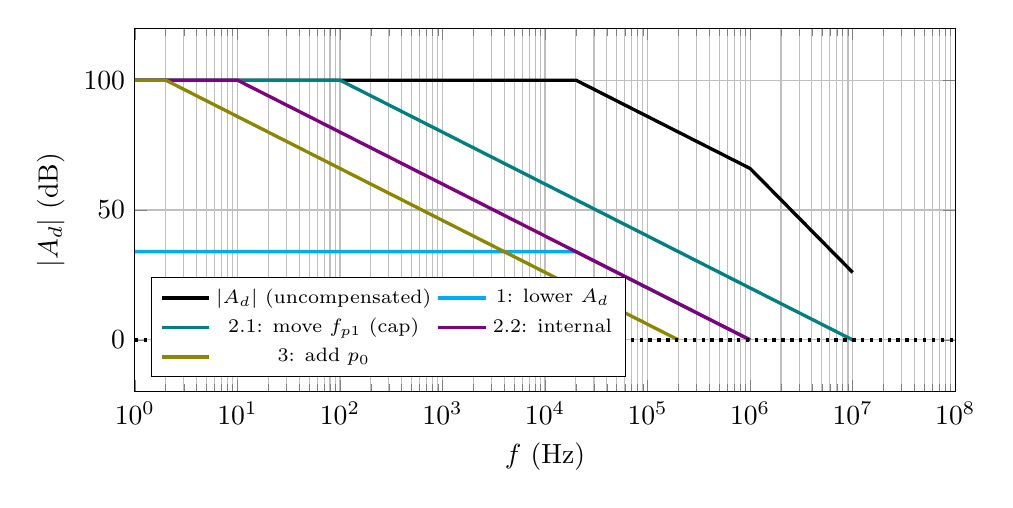
\begin{tikzpicture}
\begin{axis}[width=12cm,height=6.2cm,xmode=log,
  xlabel={$f$ (Hz)},ylabel={$|\Ad|$ (dB)},
  xmin=1,xmax=1e8,ymin=-20,ymax=120,grid=both,
  legend style={font=\scriptsize,at={(0.02,0.04)},anchor=south west,
    legend columns=2},
  every axis plot/.append style={very thick}]
\addplot[black] coordinates {(1,100)(2e4,100)(1e6,66)(1e7,26)};
\addlegendentry{$|\Ad|$ (uncompensated)}
\addplot[cyan] coordinates {(1,34)(2e4,34)(1e6,0)};
\addlegendentry{1: lower $\Ad$}
\addplot[teal] coordinates {(1,100)(100,100)(1e7,0)};
\addlegendentry{2.1: move $f_{p1}$ (cap)}
\addplot[violet] coordinates {(1,100)(10,100)(1e6,0)};
\addlegendentry{2.2: internal}
\addplot[olive] coordinates {(1,100)(2,100)(2e5,0)};
\addlegendentry{3: add $p_0$}
\addplot[black,dotted] coordinates {(1,0)(1e8,0)};
\end{axis}
\end{tikzpicture}
\caption{The four compensated open-loop gains for the running example
($\Ad0=\qty{100}{\dB}$, $f_{p1}=\qty{20}{\kilo\hertz}$,
$f_{p2}=\qty{1}{\mega\hertz}$). Here the curves are the
compensated $|\Ad|$; the loop gain $|T|$ is each curve shifted down by
$|\beta|=\qty{20}{\dB}$, so the bandwidth is where $|\Ad|=\qty{20}{\dB}$. Method
2.1 keeps the highest curve longest (best bandwidth); method 3 rolls off first
(worst); method 1 also throws the DC gain away.}
\label{fig:compensation}
\end{figure}

\begin{protocol}[Compensate the \op{}]
\begin{enumerate}[leftmargin=1.5cm]
  \item Confirm the uncompensated stage is unstable ($\phi_M<45^\circ$).
  \item If you control the board \emph{and} the part exposes compensation pins,
        use \textbf{Method 2.1}: move $f_{p1}$ to $f_{p2}/T_0$ --- best bandwidth.
  \item Otherwise choose an \textbf{internally compensated} part (\textbf{Method
        2.2}): $f_{p1}$ is fixed at $f_{p2}/\Ad0$, stable for any $A_V\ge1$, and
        the bandwidth is $f_{BW}/A_{V0}$.
  \item Avoid \textbf{Method 1} (it guts the loop gain) and \textbf{Method 3} (it
        guts the bandwidth) unless forced.
  \item Recompute $A_V(f)$ and verify the bandwidth via the GBWP (next section).
\end{enumerate}
\end{protocol}

\begin{note}
\textbf{Running example (used in all four methods below).} A non-inverting stage
of gain $A_V=10$ ($\beta=1/10$, $|\beta|=\qty{-20}{\dB}$) on an \op{} with
$\Ad0=\qty{100}{\dB}$ ($10^5$), $f_{p1}=\qty{20}{\kilo\hertz}$,
$f_{p2}=\qty{1}{\mega\hertz}$. The poles are
$n_{\mathrm{dec}}=\log_{10}(f_{p2}/f_{p1})=\log_{10}50=1.7$ decades apart, so
$|\Ad(f_{p2})|=100-20\cdot1.7=\qty{66}{\dB}$; the DC loop gain is
$T_0=\Ad0\,\beta=10^{4}$, i.e.\ $|T_0|=\qty{80}{\dB}$ and
$|T(f_{p2})|=80-34=\qty{46}{\dB}$. Uncompensated, $|T|$ crosses \qty{0}{\dB} well
past $f_{p2}$ --- unstable.
\end{note}

\subsection{Method 1 --- lower the differential gain $\Ad$}
Slide the whole $|\Ad|$ curve down (without moving any pole) until
$|T(f_{p2})|=\qty{0}{\dB}$. The required attenuation is $M=|T(f_{p2})|$.

\begin{wexample}[Method 1 on the running example]
$M=|T(f_{p2})|=\qty{46}{\dB}$, so the DC loop gain collapses from \qty{80}{\dB} to
$80-46=\qty{34}{\dB}$ --- already a poor return on the feedback. Worse, if the
manufacturer does this inside the IC it must assume the worst case $\beta=1$, so
$M=|\Ad(f_{p2})|=\qty{66}{\dB}$ and $\Ad0$ drops to \qty{34}{\dB}; used at
$A_V=10$ the loop gain is then only $34-20=\qty{14}{\dB}$. Stable, but the
feedback benefits (gain accuracy, low distortion, better $R_{in}/R_{out}$) are
almost gone.
\end{wexample}

\begin{exercise}
The same \op{} ($\Ad0=\qty{100}{\dB}$, $f_{p1}=\qty{20}{\kilo\hertz}$,
$f_{p2}=\qty{1}{\mega\hertz}$) used as a \emph{voltage follower}. Worst-case
Method~1: find $M$, the compensated $\Ad0$, and the frequency where $|T|$ now
crosses \qty{0}{\dB}.
\end{exercise}
\begin{solution}
Follower $\Rightarrow\beta=1$, so $T=\Ad$. $M=|\Ad(f_{p2})|=\qty{66}{\dB}$, giving
$\Ad0=100-66=\qty{34}{\dB}$ ($\approx50$). The pole is still at
$f_{p1}=\qty{20}{\kilo\hertz}$, so $|T|=0$ at
$f_{p1}\cdot10^{34/20}=20\,\text{k}\times50=\qty{1}{\mega\hertz}=f_{p2}$, i.e.\
$\phi_M=45^\circ$ --- just stable. But the DC loop gain is now only \qty{34}{\dB}:
the method works yet throws feedback away, so in practice it is the last choice.
\end{solution}

\subsection{Method 2.1 --- move the first pole with an external capacitor}
Add a capacitor on the dedicated compensation pins to drag $f_{p1}$ down (leaving
$f_{p2},f_{p3}$ in place) until $|T|=\qty{0}{\dB}$ lands exactly on $f_{p2}$.
Because you know \emph{your} $\beta$, you move the pole only as far as this gain
needs --- the highest possible bandwidth, $f_T=f_{p2}$. The new pole sits
$|T_0|_{\mathrm{dB}}/20$ decades below $f_{p2}$:
\[
  f_{p1}^{\,new}=f_{p2}\big/10^{\,|T_0|_{\mathrm{dB}}/20}=f_{p2}/T_0 .
\]

\begin{wexample}[Method 2.1 on the running example]
$f_{p1}^{\,new}=f_{p2}/10^{80/20}=10^{6}/10^{4}=\qty{100}{\hertz}$. The DC loop
gain stays at the full \qty{80}{\dB} and the closed-loop bandwidth is the best
attainable, $f_T=f_{p2}=\qty{1}{\mega\hertz}$. The price: an external capacitor
and pins that are not always available.
\end{wexample}

\begin{exercise}
The same \op{}, now at $A_V=100$. Where must Method~2.1 place $f_{p1}^{\,new}$,
and what DC loop gain survives?
\end{exercise}
\begin{solution}
$\beta=1/100$, $|T_0|=100-40=\qty{60}{\dB}$ ($10^{3}$). Move the pole to
$f_{p1}^{\,new}=f_{p2}/10^{60/20}=10^{6}/10^{3}=\qty{1}{\kilo\hertz}$. The DC loop
gain is the full \qty{60}{\dB} --- Method~2.1 always keeps it; that is its appeal.
\end{solution}

\subsection{Method 2.2 --- use an internally compensated \op{}}
When you cannot add a capacitor, pick a part the manufacturer has already
compensated for the \emph{worst case} $\beta=1$ (the follower): the internal cap
moves $f_{p1}$ until $|\Ad(f_{p2})|=\qty{0}{\dB}$, i.e.
\[
  f_{p1}^{\,new}=f_{p2}\big/10^{\,|\Ad0|_{\mathrm{dB}}/20}=f_{p2}/\Ad0 .
\]
It is then stable for \emph{any} $A_V\ge1$. This is the everyday choice
(LM741, TL08x, \dots): trivial to use and the full DC loop gain is kept; only the
bandwidth shrinks as gain rises.

\begin{wexample}[Method 2.2 on the running example, plus a datasheet]
$f_{p1}^{\,new}=f_{p2}/\Ad0=10^{6}/10^{5}=\qty{10}{\hertz}$, lower than
Method~2.1's \qty{100}{\hertz} (because it must also cover the follower) --- hence
less bandwidth, but unconditionally stable. From a real datasheet:
$\Ad0=\qty{400}{k}$ (\qty{112}{\dB}), $f_{p2}=\qty{1}{\mega\hertz}\Rightarrow
f_{p1}^{\,new}=10^{6}/(400\times10^{3})=\qty{2.5}{\hertz}$, and the measured phase
margin is $\phi_M=90^\circ$ --- well past the $45^\circ$ minimum (and even larger
at $A_V>1$).
\end{wexample}

\begin{exercise}
The same internally compensated part is used once as a follower and once at
$A_V=10$. Does $f_{p1}^{\,new}$ change between the two uses? What \emph{does}
change?
\end{exercise}
\begin{solution}
No --- $f_{p1}^{\,new}=f_{p2}/\Ad0$ is fixed in the factory for the worst case
$\beta=1$, so it is the same part however you wire it. What changes is the
\textbf{bandwidth}: $f_T=f_{BW}/A_{V0}$, so the follower gets the full
$f_T=f_{BW}=f_{p2}$ while the $A_V=10$ stage gets only $f_{p2}/10$. Higher gain
always costs bandwidth here --- that is the GBWP (next section).
\end{solution}

\subsection{Method 3 --- add a new dominant pole $p_0$}
Introduce a brand-new low-frequency pole $p_0$ below $f_{p1}$ so it becomes
dominant and the old $f_{p1}$ slips into the role of ``second pole''. Place it so
$|T|$ is already at \qty{0}{\dB} by the \emph{original} first pole:
\[
  f_{p0}=f_{p1}\big/10^{\,|T_0|_{\mathrm{dB}}/20}=f_{p1}/T_0 .
\]
Because the rolloff now starts so early, this gives the \emph{worst} bandwidth of
all.

\begin{wexample}[Method 3 on the running example]
$f_{p0}=f_{p1}/T_0=20\,\text{k}/10^{4}=\qty{2}{\hertz}$. The DC loop gain is kept
(\qty{80}{\dB}, good feedback), but the bandwidth is crushed to
$f_T=f_{p1}=\qty{20}{\kilo\hertz}$ --- two decades below Method~2.1. Rarely used
for exactly this reason.
\end{wexample}

\begin{exercise}
The same \op{} at $A_V=100$. Where does Method~3 place $p_0$? Where would
Method~2.1 instead put the moved first pole, and why does Method~3 leave so much
less usable bandwidth?
\end{exercise}
\begin{solution}
$|T_0|=\qty{60}{\dB}$ ($10^{3}$): Method~3 sets $f_{p0}=f_{p1}/10^{3}=
20\,\text{k}/1000=\qty{20}{\hertz}$, while Method~2.1 would put the moved pole at
$f_{p2}/10^{3}=\qty{1}{\kilo\hertz}$. Both keep the full \qty{60}{\dB} of DC loop
gain, but Method~3's dominant pole sits a factor $f_{p1}/f_{p2}=1/50$ lower, so
its closed-loop bandwidth is about $50\times$ smaller. Method~3 protects the
feedback but pays the heaviest bandwidth penalty.
\end{solution}

\bigskip
The four methods at the running gain $A_V=10$ side by side:

\begin{center}\small
\begin{tabular}{@{}lllll@{}}
\toprule
\textbf{Method} & \textbf{New dominant pole} & \textbf{DC loop gain $T_0$}
  & \textbf{Bandwidth $f_T$} & \textbf{When to use}\\
\midrule
1\ \ lower $\Ad$        & $f_{p1}$ unmoved (\qty{20}{\kilo\hertz}) & \qty{14}{\dB} (gutted) & \qty{100}{\kilo\hertz} & avoid\\
2.1\ external cap       & \qty{100}{\hertz}  & \qty{80}{\dB} (full) & \qty{1}{\mega\hertz}   & best, if pins exist\\
2.2\ internal           & \qty{10}{\hertz}   & \qty{80}{\dB} (full) & \qty{100}{\kilo\hertz} & default / easiest\\
3\ \ add $p_0$          & \qty{2}{\hertz}    & \qty{80}{\dB} (full) & \qty{20}{\kilo\hertz}  & rare (worst BW)\\
\bottomrule
\end{tabular}
\end{center}

\noindent Note how Methods 1 and 2.2 reach the \emph{same} bandwidth
(\qty{100}{\kilo\hertz}) yet Method 2.2 keeps \qty{80}{\dB} of loop gain against
Method 1's \qty{14}{\dB}: that is why nobody uses Method 1.

\begin{note}
\textbf{Inverting stages.} An inverting amplifier has the same feedback network as
the non-inverting one, hence the same $\beta=R_1/(R_1+R_2)$ and the same loop gain
$T=\Ad\beta$ --- stability does not depend on where $V_{in}$ connects. Analyse it
as a non-inverting stage of gain $1/\beta$. Example: $A_V=-2$ needs $R_2/R_1=2$,
so $\beta=\tfrac{R_1}{R_1+R_2}=\tfrac13$ and you study the stability of a
non-inverting stage of gain $1/\beta=3$.
\end{note}

\section{Bandwidth from the Gain--Bandwidth Product}
Take an internally compensated part (Method 2.2): a single dominant pole at $f_0$
makes the closed loop look like one pole,
\[
  A_V(f)\simeq\frac1\beta\,\frac{1}{1+jf/(\Ad0\beta f_0)},\qquad
  f_T=\Ad0\,\beta\,f_0=\frac{f_{BW}}{A_{V0}},
\]
with $f_{BW}=\Ad0 f_0$ a \emph{constant} of the device (Appendix~\ref{app:gbwp}).
So gain and bandwidth trade one-for-one: doubling the gain halves the bandwidth.
The follower ($A_{V0}=1$) gets the whole $f_{BW}$. (The GBWP shortcut applies only
to internally compensated parts; with Method 2.1 the cap is retuned per gain and
$f_T=f_{p2}$ always.)

\begin{protocol}[Bandwidth via GBWP]
\begin{enumerate}[leftmargin=1.5cm]
  \item $f_T=\text{GBWP}/A_{V0}$ (for an inverting stage use the equivalent
        non-inverting gain $A_{V0}=|A_{inv}|+1$).
  \item If $f_T\ge f_C$ (the required bandwidth), done.
  \item Else either pick a faster \op{} (GBWP $\ge A_{V0}f_C$), \emph{or} split
        the gain across cascaded stages so each stage keeps a higher $f_T$.
\end{enumerate}
\end{protocol}

\begin{wexample}[GBWP, pass and fail]
GBWP $=\qty{1}{\mega\hertz}$, want $f_C=\qty{40}{\kilo\hertz}$.
\emph{(1)} $A_{V0}=12\Rightarrow f_T=10^6/12=\qty{83.3}{\kilo\hertz}>f_C$ --- meets
spec. \emph{(2)} $A_{V0}=100\Rightarrow f_T=\qty{10}{\kilo\hertz}<f_C$ --- fails.
Fix it by choosing a part with GBWP $\ge100\times40\,\text{k}=\qty{4}{\mega\hertz}$,
\emph{or} by cascading two $\times10$ stages: each has
$f_T'=10^6/10=\qty{100}{\kilo\hertz}$, the product gain is $100$, and the combined
bandwidth (slightly under \qty{100}{\kilo\hertz}) clears the spec.
\end{wexample}

\begin{exercise}
A non-inverting stage needs $A_{V0}=25$ and a bandwidth $f_C=\qty{50}{\kilo\hertz}$
from a part with GBWP $=\qty{1}{\mega\hertz}$. Does it meet spec? Give two fixes.
\end{exercise}
\begin{solution}
$f_T=10^6/25=\qty{40}{\kilo\hertz}<\qty{50}{\kilo\hertz}$ --- \textbf{fails}.
\emph{(i)} Use a faster \op{}: GBWP $\ge25\times50\,\text{k}=\qty{1.25}{\mega\hertz}$.
\emph{(ii)} Cascade two $\times5$ stages: each $f_T'=10^6/5=\qty{200}{\kilo\hertz}$,
product gain $25$, combined bandwidth just under \qty{200}{\kilo\hertz} --- spec
met with margin.
\end{solution}

\section{Slew rate}
Bandwidth is a \emph{small-signal} limit. The \textbf{slew rate} is the
\emph{large-signal} ceiling on how fast the output can move,
\[
  \text{SR}=\max\frac{\mathrm{d}v_{out}}{\mathrm{d}t}=\frac{I_s}{C_c},
\]
set by the largest current $I_s$ the \op{} can push into its compensation
capacitor $C_c$ ($\Delta V_C=\tfrac{1}{C_c}\!\int\! i\,\mathrm{d}t=\tfrac{I_s}{C_c}t$
for a constant current). Feed an ideal step and the output ramps at this fixed
slope instead of following.

\begin{note}
\textbf{Bandwidth vs slew rate on a step.} Both come from the same internal
capacitances but answer different questions. The small-signal rise time
$t_{10\text{--}90}=2.2\tau=0.35/\text{BW}$ (with $\tau=1/2\pi\,\text{BW}$) is set by
the bandwidth and is \emph{independent} of the step height. The slewing rise time
$t_{10\text{--}90}=0.8\,V_H/\text{SR}$ \emph{grows} with the step height $V_H$.
Small steps are bandwidth-limited; large steps are slew-limited.
\end{note}

For a sinusoid $v_{out}=V_p\sin\omega t$ the steepest slope is $V_p\omega$, so the
output stays undistorted only while
\[
  V_p\,\omega\le\text{SR}\;\Longrightarrow\;V_p\le\frac{\text{SR}}{2\pi f}
  \quad\text{(full-power bandwidth).}
\]
The usable amplitude therefore falls off as $1/f$; at low frequency it is capped
instead by the output dynamic range.

\begin{protocol}[Bandwidth vs slew-rate limit]
\begin{enumerate}[leftmargin=1.5cm]
  \item Max gain from GBWP: $G_{\max}=\text{GBWP}/f_0$.
  \item Max undistorted amplitude from SR: $V_p<\text{SR}/(2\pi f_0)$.
  \item Whichever bound bites first --- gain (bandwidth) or amplitude (slew) ---
        limits the design; if both are respected there is no limitation.
\end{enumerate}
\end{protocol}

\begin{wexample}[Full-power bandwidth of an LM741]
$\text{SR}=\qty{0.5}{\volt\per\micro\second}=\qty{500}{\kilo\volt\per\second}$.
The largest \emph{undistorted} frequency depends on the amplitude:
$f=\text{SR}/(2\pi V_p)$. For the full $\pm\qty{12}{\volt}$ swing
$f=5\times10^5/(2\pi\cdot12)=\qty{6.63}{\kilo\hertz}$; for $\pm\qty{10}{\volt}$,
\qty{7.96}{\kilo\hertz}; $\pm\qty{5}{\volt}$, \qty{15.9}{\kilo\hertz};
$\pm\qty{1}{\volt}$, \qty{79.6}{\kilo\hertz}. Smaller signals can run faster.
\end{wexample}

\begin{wexample}[TL082: which limit bites?]
$\text{SR}=\qty{13}{\volt\per\micro\second}$, GBWP $=\qty{4}{\mega\hertz}$,
$f_0=\qty{400}{\kilo\hertz}$. $G_{\max}=4\times10^6/4\times10^5=10$;
$V_p<13\times10^6/(2\pi\cdot4\times10^5)=\qty{5.17}{\volt}$. So: $V_p<\qty{5.17}{\volt}$
but gain $>10$ $\Rightarrow$ bandwidth limits; gain $<10$ but
$V_p>\qty{5.17}{\volt}$ $\Rightarrow$ slew rate limits; both respected
$\Rightarrow$ no limitation.
\end{wexample}

\begin{exercise}
An LM741 ($\text{SR}=\qty{0.5}{\volt\per\micro\second}$) must output a
\qty{10}{\kilo\hertz} sine. (a)~What is the largest amplitude $V_p$ free of
slewing? (b)~If a $\qty{10}{\volt}$ peak is required, above what frequency does it
slew?
\end{exercise}
\begin{solution}
(a) $V_p\le\text{SR}/(2\pi f)=5\times10^{5}/(2\pi\cdot10^{4})=\qty{7.96}{\volt}$.
(b) $f\le\text{SR}/(2\pi V_p)=5\times10^{5}/(2\pi\cdot10)=\qty{7.96}{\kilo\hertz}$,
so a \qty{10}{\volt} peak already slews at \qty{10}{\kilo\hertz}; drop the
amplitude or use a faster part (e.g.\ a TL082).
\end{solution}

%=======================================================================
\chapter{Applications}\label{ch:apps}
%=======================================================================

\section{The audio amplifier (placing poles and zeros)}
A practical amplifier has a finite pass band $[f_L,f_H]$ and a chosen input
impedance. The non-inverting stage gets three capacitors: $C_3$ blocks input DC,
$C_1$ sets the DC gain to 1 (kills offset amplification), $C_2$ rolls off the
high end. Analyse it at three frequencies (Appendix~\ref{app:freqresp}).

\begin{protocol}[Design the audio amplifier]
\begin{enumerate}[leftmargin=1.5cm]
  \item \textbf{DC} (caps open): input disconnected, gain to offset is 1 --- good.
  \item \textbf{Pass band} (C$_1$,C$_3$ short, C$_2$ open): $R_{in}=R_3$; set
        $R_3=R_{in}^{spec}$, then $R_2=R_3$ (offset), then
        $R_1=R_2/(A_{V0}-1)$.
  \item \textbf{High end}: pole $f_H=1/(2\pi R_2C_2)\Rightarrow C_2$.
  \item \textbf{Low end}: poles $f_{p1}=1/(2\pi R_1C_1)=f_L$ and
        $f_{p3}=1/(2\pi R_3C_3)$ (place a decade below $f_L$) $\Rightarrow
        C_1,C_3$.
  \end{enumerate}
\end{protocol}

\begin{figure}[h]\centering
\begin{circuitikz}[scale=0.92,transform shape]
  \node[op amp] (oa){};                  % default orientation: (-) on top, (+) on bottom
  \coordinate (ninv) at (oa.+);          % non-inverting input (bottom)
  \coordinate (inv)  at (oa.-);          % inverting input (top); alias avoids the '-' path bug
  % --- output ---
  \draw (oa.out) -- ++(1.3,0) coordinate(O) to[short,-o] ++(0.35,0) node[right]{$v_{out}$};
  % --- (+) input: v_in --C3--> node P, R3 to ground ---
  \draw (ninv) -- ++(-0.7,0) coordinate(P);
  \draw (P) to[C=$C_3$,-o] ++(-1.8,0) node[left]{$v_{in}$};
  \draw (P) to[R=$R_3$] ++(0,-2.0) node[ground]{};
  % --- (-) input node M ---
  \draw (inv) -- ++(-0.7,0) coordinate(M);
  % gain leg (forces unity DC gain): rail left, above the input network, then R1 + C1 to ground
  \draw (M) -- ++(-3.1,0) coordinate(G);
  \draw (G) to[R,l_=$R_1$] ++(0,-1.5) to[C,l_=$C_1$] ++(0,-1.3) node[ground]{};
  % --- feedback R2 || C2, kept horizontal over the top to the output ---
  \draw (M) -- ++(0,1.5) coordinate(a);  \draw (a)  to[R=$R_2$] (a  -| O) coordinate(b);  \draw (b)  -- (O);
  \draw (M) -- ++(0,2.5) coordinate(a2); \draw (a2) to[C=$C_2$] (a2 -| O) coordinate(b2); \draw (b2) -- (b);
\end{circuitikz}
\caption{Audio amplifier: $C_3$ AC-couples the input, $C_1$ forces unity DC gain,
$C_2$ sets the upper cutoff.}
\label{fig:audio}
\end{figure}

\begin{wexample}[Full audio design]
$f_L=\qty{20}{\hertz}$, $f_H=\qty{20}{\kilo\hertz}$, $A_{V0}=10$,
$R_{in}=\qty{100}{\kilo\ohm}$. Then $R_3=R_2=\qty{100}{\kilo\ohm}$,
$R_1=R_2/(A_{V0}-1)=100/9\approx\qty{12}{\kilo\ohm}$. Caps:
$C_2=1/(2\pi R_2 f_H)=\qty{80}{\pico\farad}$,
$C_1=1/(2\pi R_1 f_L)=\qty{663}{\nano\farad}$,
$C_3=1/(2\pi R_3 f_{p3})$ with $f_{p3}=\qty{2}{\hertz}\Rightarrow\qty{800}{\nano\farad}$.
\end{wexample}

\begin{exercise}
Design the same topology for $f_L=\qty{50}{\hertz}$, $f_H=\qty{15}{\kilo\hertz}$,
$A_{V0}=20$, $R_{in}=\qty{47}{\kilo\ohm}$ (place $f_{p3}$ a decade below $f_L$).
\end{exercise}
\begin{solution}
$R_3=R_2=\qty{47}{\kilo\ohm}$;
$R_1=R_2/(A_{V0}-1)=47/19\approx\qty{2.5}{\kilo\ohm}$ (nearest E12
\qty{2.7}{\kilo\ohm} realises $A_{V0}=18.4$; keep \qty{2.5}{\kilo\ohm} if the
gain matters). Caps: $C_2=1/(2\pi R_2f_H)=\qty{226}{\pico\farad}\to
\qty{220}{\pico\farad}$; $C_1=1/(2\pi R_1f_L)=\qty{1.27}{\micro\farad}\to
\qty{1.2}{\micro\farad}$; $f_{p3}=\qty{5}{\hertz}$:
$C_3=1/(2\pi R_3f_{p3})=\qty{677}{\nano\farad}\to\qty{680}{\nano\farad}$.
\end{solution}

\section{Generalised adder/subtractor}
To realise $v_{out}=\sum A_j' v_j' - \sum A_i'' v_i''$, feed the ``$+$'' inputs to
the non-inverting terminal and the ``$-$'' inputs to the inverting terminal,
each through $R=R_f/A$.

\begin{protocol}[Generalised adder/subtractor]
\begin{enumerate}[leftmargin=1.5cm]
  \item Fix $R_f$. For every coefficient set its resistor $R=R_f/|A|$
        ($-$ signs $\to$ inverting side, $+$ signs $\to$ non-inverting side).
  \item Balance: require $\bigl(1+\sum A_i''\bigr)/\sum A_j'=1$. If $>1$ add a
        resistor to ground on the $+$ side; if $<1$ add one on the $-$ side.
        This also equalises the input resistances (offset minimised).
\end{enumerate}
\end{protocol}

\begin{wexample}[$v_{out}=2v_1'+5v_2'$]
$\sum A_j'=7$, $\sum A_i''=0$, so $(1+0)/7<1$: add a resistor on the $-$ side
with $A_1''=6$. Resistors: $R_1'=R_f/2$, $R_2'=R_f/5$, $R_1''=R_f/6$. Both input
terminals then see $R_f/7$ --- offsets minimised.
\end{wexample}

\begin{exercise}
Realise (a) $v_{out}=-2v_1-3v_2-4v_3$ and (b) the difference
$v_{out}=6(v_1'-v_1'')$. Give the resistors and the balancing element.
\end{exercise}
\begin{solution}
(a) All inverting: $R_i''=R_f/2,R_f/3,R_f/4$; here $(1+9)/0$ diverges, so add a
$+$-side resistor with $A_1'=10$, $R_1'=R_f/10$ (the $+$ node is not simply
grounded). (b) $A_1'=A_1''=6$: $R_1'=R_1''=R_f/6$; $(1+6)/6>1$ $\Rightarrow$ add
$A_2'=1$, $R_2'=R_f$ to ground on the $+$ side. It is a differential amplifier.
\end{solution}

\section{The integrator}\label{sec:integrator}
Replace the inverting amp's feedback resistor with a capacitor:
$v_{out}(t)=-\frac1{RC}\int v_{in}\,\mathrm{d}t$ (pole at the origin). A constant
input gives a ramp; a square wave gives a triangle of peak-to-peak
$V_{in}\,(T/2)/RC$; a sine comes out scaled by $1/(\omega RC)$ and shifted by
$+90^\circ$ (on top of the inversion).

\emph{Why the textbook integrator fails as drawn.} At DC the capacitor is an
open circuit, so there is \emph{no} feedback at all: the input offset voltage
and bias current are integrated unopposed and the output drifts (``winds up'')
to a rail within seconds. The fix is a resistor $R_2$ in parallel with $C$: it
restores DC feedback with gain $-R_2/R$, turning the pole at the origin into a
pole at $f_p=1/(2\pi R_2C)$. The circuit then integrates only for $f\gg f_p$ ---
which is all a real application needs.

\begin{protocol}[Design a practical integrator]
\begin{enumerate}[leftmargin=1.5cm]
  \item Set $RC$ from the job: triangle from a square wave,
        $V_{pp,tri}=V_{in}\,\dfrac{T/2}{RC}$; or gain at the working frequency,
        $|A(f)|=1/(2\pi fRC)$.
  \item Split $RC$: choose $R$ well above the source resistance, then
        $C=RC/R$.
  \item Add $R_2=A_{DC}\,R$ across $C$, with $A_{DC}$ the largest tolerable DC
        (offset) gain; check that the pole $f_p=1/(2\pi R_2C)$ sits at least a
        decade below the lowest working frequency.
  \item Check the residual DC output,
        $\approx V_{\!OFF}(1+R_2/R)+I_{BIAS}R_2$ (and add $R_3=R\Vert R_2$ on
        the $+$ input as usual, \S\ref{sec:offset}).
\end{enumerate}
\end{protocol}

\begin{figure}[h]\centering
\begin{circuitikz}[scale=0.85,transform shape]
  \draw (0,0) node[op amp, noinv input up] (oa){};
  \draw (oa.-) -- ++(-1.0,0) coordinate(M);
  \draw (M) to[R=$R$,-o] ++(-2.4,0) node[left]{$v_{in}$};
  \draw (oa.+) -- ++(-0.6,0) node[ground]{};
  \draw (oa.out) -- ++(1.3,0) coordinate(O) to[short,-o] ++(0.2,0) node[right]{$v_{out}$};
  \draw (M) -- ++(0,1.7) coordinate(a);
  \draw (a) to[C=$C$] (a -| O) coordinate(b); \draw (b) -- (O);
\end{circuitikz}
\caption{Inverting integrator.}
\label{fig:integrator}
\end{figure}

\begin{wexample}[Square wave $\to$ triangle]
Input: $\pm\qty{1}{\volt}$ square wave at \qty{1}{\kilo\hertz}; wanted: a
\qty{2}{\volt} peak-to-peak triangle. During each half period
($T/2=\qty{0.5}{\milli\second}$) the constant $\pm\qty{1}{\volt}$ input ramps
the output by $V_{in}(T/2)/RC$, so
$2=1\times0.5\,\text{ms}/RC\Rightarrow RC=\qty{0.25}{\milli\second}$. Pick
$C=\qty{10}{\nano\farad}\Rightarrow R=\qty{25}{\kilo\ohm}$ (E12
\qty{27}{\kilo\ohm} gives $V_{pp}=\qty{1.85}{\volt}$, $-7\%$). DC stability:
accept $A_{DC}=100$, so $R_2=100R=\qty{2.5}{\mega\ohm}$ and
$f_p=1/(2\pi R_2C)=\qty{6.4}{\hertz}$ --- more than two decades below
\qty{1}{\kilo\hertz}, so the triangle is unaffected.
\end{wexample}

\begin{exercise}
(a) Feed the integrator above ($RC=\qty{0.25}{\milli\second}$) a
\qty{100}{\milli\volt} sine at \qty{500}{\hertz}: output amplitude and phase?
(b) Remove $R_2$ and take $I_{BIAS}=\qty{100}{\nano\ampere}$: starting from
$0$, how long until the output hits a \qty{12}{\volt} rail?
\end{exercise}
\begin{solution}
(a) $|A|=1/(2\pi fRC)=1/(2\pi\times500\times2.5\times10^{-4})=1.27$: output
\qty{127}{\milli\volt}, at $-90^\circ+180^\circ=+90^\circ$ (integration plus
inversion). (b) With no DC feedback $I_{BIAS}$ flows straight into $C$:
$\mathrm{d}v/\mathrm{d}t=I/C=10^{-7}/10^{-8}=\qty{10}{\volt\per\second}$, so the
rail arrives in $\approx\qty{1.2}{\second}$ --- the wind-up that $R_2$ exists to
stop.
\end{solution}

%=======================================================================
\chapter{The Operational Amplifier as a comparator}\label{ch:comp}
%=======================================================================

Without negative feedback the \op{} saturates: it becomes a \textbf{comparator},
output $V_{OH}$ or $V_{OL}$. This chapter climbs the whole ladder: the bare
comparator and why noise makes it chatter (\S\ref{sec:plaincomp}), the two
Schmitt-trigger topologies that fix it
(\S\ref{sec:invschmitt}--\ref{sec:nischmitt}), and the two oscillators built
from them --- the astable square-wave generator and the triangle/square
generator.

\section{The bare threshold comparator}\label{sec:plaincomp}
Open the loop and the \op{} becomes a one-bit analog-to-digital converter:
with $\Ad\sim10^5$, a differential input of a few tens of \unit{\micro\volt}
already rails the output, so for any practical input
\[
  v_{out}=\begin{cases}V_{OH} & v_+>v_-\,,\\[2pt] V_{OL} & v_+<v_-\,.\end{cases}
\]
Which terminal carries the signal fixes the polarity. \textbf{Non-inverting}
($v_{in}$ on $+$, $V_{REF}$ on $-$): output high for $v_{in}>V_{REF}$.
\textbf{Inverting} ($v_{in}$ on $-$, $V_{REF}$ on $+$): output high for
$v_{in}<V_{REF}$. Either way the output is binary, and the levels can be made
compatible with TTL or any other logic standard.

\begin{figure}[h]\centering
\begin{tabular}{cc}
\begin{tikzpicture}[scale=0.8]
  \draw[->](-0.3,0)--(3.4,0) node[right]{$v_{in}$};
  \draw[->](0,-0.3)--(0,2.4) node[above]{$v_{out}$};
  \draw[very thick,accent] (0.2,0.2)--(1.7,0.2)--(1.7,2)--(3.1,2);
  \node[below] at (1.7,0){$V_{REF}$};
  \node[left] at (0,2){$V_{OH}$}; \node[left] at (0,0.2){$V_{OL}$};
\end{tikzpicture}
&
\begin{tikzpicture}[scale=0.8]
  \draw[->](-0.3,0)--(3.4,0) node[right]{$v_{in}$};
  \draw[->](0,-0.3)--(0,2.4) node[above]{$v_{out}$};
  \draw[very thick,accent] (0.2,2)--(1.7,2)--(1.7,0.2)--(3.1,0.2);
  \node[below] at (1.7,0){$V_{REF}$};
  \node[left] at (0,2){$V_{OH}$}; \node[left] at (0,0.2){$V_{OL}$};
\end{tikzpicture}
\\[2pt]
{\footnotesize Non-inverting: high for $v_{in}>V_{REF}$} &
{\footnotesize Inverting: high for $v_{in}<V_{REF}$}
\end{tabular}
\caption{Transfer characteristics of the bare comparator: a single step at
$V_{REF}$, with polarity set by which terminal carries the signal.}
\label{fig:plaincomp}
\end{figure}

\begin{warning}
Near the threshold the bare comparator is \emph{extremely} sensitive to noise
(supply ripple, temperature drift, electromagnetic interference). Model the
disturbance as a random signal of maximum amplitude $\pm N_A$ riding on
$v_{in}$: the output is guaranteed only for $|v_{in}-V_{REF}|>N_A$. Inside the
band $V_{REF}\pm N_A$ the output depends on the instantaneous noise value and
shows random oscillations (``chatter''). Hysteresis (next section) is the
cure.
\end{warning}

\begin{protocol}[Analyse a bare comparator]
\begin{enumerate}[leftmargin=1.5cm]
  \item Identify the terminals: which input carries $v_{in}$, which $V_{REF}$
        (generate $V_{REF}$ with a divider if needed).
  \item Apply the rule $v_{out}=V_{OH}$ iff $v_d=v_+-v_->0$; sketch the
        transfer characteristic (one step at $V_{REF}$, polarity from step~1).
  \item Translate to the time domain: the output toggles at every crossing of
        $V_{REF}$ by $v_{in}$.
  \item \textbf{Noise check}: the output is undefined while
        $|v_{in}-V_{REF}|<N_A$; estimate how long each crossing spends in that
        band. If chatter is unacceptable, switch to a Schmitt trigger with
        $\Delta V_S>2N_A$.
\end{enumerate}
\end{protocol}

\begin{wexample}[Squaring-up a triangle wave]
A non-inverting comparator with $V_{REF}=\qty{2}{\volt}$ receives a
0--\qty{4}{\volt}, \qty{1}{\kilo\hertz} triangle. Output: a square wave, high
while $v_{in}>\qty{2}{\volt}$, i.e.\ \qty{50}{\percent} duty cycle. Now let
noise of $N_A=\qty{0.1}{\volt}$ ride on the input. The triangle slews at
$\qty{4}{\volt}/\qty{0.5}{\milli\second}=\qty{8}{\volt\per\milli\second}$, so
each crossing spends $2N_A/(\qty{8}{\volt\per\milli\second})=
\qty{25}{\micro\second}$ inside the undefined band $\qty{1.9}{\volt}$--$\qty{2.1}{\volt}$
--- a \qty{25}{\micro\second} burst of random edges, twice per period. A
Schmitt trigger with $\Delta V_S>\qty{0.2}{\volt}$ removes them.
\end{wexample}

\begin{exercise}
Build an inverting comparator on a single \qty{5}{\volt} supply.
(a)~Choose an E12 divider from the rail so that $V_{REF}=\qty{2.0}{\volt}$.
(b)~State the output rule. (c)~With $N_A=\qty{50}{\milli\volt}$, give the input
band where the output is undefined, and the minimum hysteresis a Schmitt
replacement would need.
\end{exercise}
\begin{solution}
(a) $V_{REF}=5\,R_b/(R_a+R_b)=\qty{2}{\volt}\Rightarrow R_a/R_b=1.5$: take
$R_a=\qty{15}{\kilo\ohm}$ (top), $R_b=\qty{10}{\kilo\ohm}$ (bottom) --- both
E12, exact. (b) Inverting: $v_{out}=V_{OH}$ for $v_{in}<\qty{2.0}{\volt}$,
$V_{OL}$ for $v_{in}>\qty{2.0}{\volt}$. (c) Undefined for
$\qty{1.95}{\volt}<v_{in}<\qty{2.05}{\volt}$; the design rule
$\Delta V_S>2N_A$ requires at least \qty{0.1}{\volt} of hysteresis.
\end{solution}

\section{Inverting Schmitt trigger}\label{sec:invschmitt}
Positive feedback makes $v_+$ depend on $v_{out}$:
\[
  v_+=V_{REF}\,\frac{R_2}{R_1+R_2}+v_{out}\,\frac{R_1}{R_1+R_2},
\]
so the trip point seen by $v_{in}$ ($=v_-$) differs between the two output
states. With the output high, the comparator flips when $v_{in}$ \emph{rises}
through $V_{S1}$; with it low, it flips back when $v_{in}$ \emph{falls} through
$V_{S2}$ (derivation Appendix~\ref{app:osc}):
\[
  V_{S1,2}=V_{REF}\,\frac{R_2}{R_1+R_2}+V_{OH,OL}\,\frac{R_1}{R_1+R_2},\qquad
  \Delta V_S=V_{S1}-V_{S2}=\frac{R_1}{R_1+R_2}\,(V_{OH}-V_{OL}).
\]
The \emph{mean} of the hysteresis is
\[
  V_{S,avg}=\frac{V_{S1}+V_{S2}}{2}
   =V_{REF}\,\frac{R_2}{R_1+R_2}+\frac{V_{OH}+V_{OL}}{2}\,\frac{R_1}{R_1+R_2}.
\]

\begin{warning}
$V_{REF}$ is \textbf{not} the mean of the thresholds: $V_{S,avg}$ contains an
output-level term $\frac{V_{OH}+V_{OL}}2\frac{R_1}{R_1+R_2}$ on top of the
attenuated $V_{REF}$. Even for symmetric levels ($V_{OL}=-V_{OH}$), where that
term vanishes, $V_{S,avg}=V_{REF}\frac{R_2}{R_1+R_2}\neq V_{REF}$. Centring
the hysteresis is a design step, not a freebie.
\end{warning}

\begin{protocol}[Design a Schmitt trigger]
\begin{enumerate}[leftmargin=1.5cm]
  \item Assume $v_{out}\in\{V_{OH},V_{OL}\}$ and $i_\pm=0$; write $v_+$ as the
        divider of $V_{REF}$ and $v_{out}$.
  \item Solve the two switching points $V_{S1}$ (where a high output flips low)
        and $V_{S2}$.
  \item From the required $\Delta V_S=V_{S1}-V_{S2}$ get $R_2/R_1$; from one
        threshold (or from $V_{S,avg}$) get $V_{REF}$. Choose absolute
        $R_1,R_2$ by other constraints.
  \item Ensure $\Delta V_S>2N_A$ (twice the noise amplitude).
  \end{enumerate}
\end{protocol}

\begin{figure}[h]\centering
\begin{tabular}{cc}
\begin{circuitikz}[scale=0.8,transform shape]
  \draw (0,0) node[op amp] (oa){};   % default: - top, + bottom
  \draw (oa.-) to[short,-o] ++(-1.6,0) node[left]{$v_{in}$};
  \draw (oa.+) -- ++(-0.8,0) coordinate(P);
  \draw (P) to[R=$R_2$,-o] ++(-2.2,0) node[left]{$V_{REF}$};
  \draw (oa.out) -- ++(1.3,0) coordinate(O) to[short,-o] ++(0.2,0) node[right]{$v_{out}$};
  \draw (P) -- ++(0,-1.8) coordinate(a);
  \draw (a) to[R=$R_1$] (a -| O) coordinate(b); \draw (b) -- (O);
\end{circuitikz}
&
\begin{tikzpicture}[scale=0.8]
  \draw[->](-0.3,0)--(3.4,0) node[right]{$v_{in}$};
  \draw[->](0,-0.3)--(0,2.4) node[above]{$v_{out}$};
  \draw[very thick,accent] (0.3,2)--(2.4,2);
  \draw[very thick,accent] (1.0,0.2)--(3.0,0.2);
  \draw[very thick,accent,->] (2.4,2)--(2.4,0.2);
  \draw[very thick,accent,->] (1.0,0.2)--(1.0,2);
  \node[below] at (2.4,0){$V_{S1}$}; \node[below] at (1.0,0){$V_{S2}$};
  \node[left] at (0,2){$V_{OH}$}; \node[left] at (0,0.2){$V_{OL}$};
\end{tikzpicture}
\\[2pt]
{\footnotesize Inverting Schmitt trigger} & {\footnotesize Hysteresis characteristic}
\end{tabular}
\caption{Positive feedback creates two thresholds; the output is immune to noise
smaller than $\Delta V_S=V_{S1}-V_{S2}$.}
\label{fig:schmitt}
\end{figure}

\begin{wexample}[Inverting Schmitt]
$V_{OL}=0$, $V_{OH}=\qty{5}{\volt}$, $V_{S1}=\qty{3}{\volt}$,
$V_{S2}=\qty{1.5}{\volt}$. $\Delta V_S=\qty{1.5}{\volt}=5\cdot\frac{R_1}{R_1+R_2}
\Rightarrow R_2=\tfrac{7}{3}R_1$. From $V_{S1}=V_{REF}\frac{R_2}{R_1+R_2}
+V_{OH}\frac{R_1}{R_1+R_2}=0.7V_{REF}+1.5=3\Rightarrow V_{REF}=\qty{2.14}{\volt}$.
Pick $R_1=\qty{10}{\kilo\ohm}$, $R_2=\qty{23.3}{\kilo\ohm}$.
Check the trap: $V_{S,avg}=\tfrac{3+1.5}{2}=\qty{2.25}{\volt}$ while
$V_{REF}=\qty{2.14}{\volt}$ --- the reference is \emph{not} the centre of the
hysteresis.
\end{wexample}

\begin{exercise}
Symmetric Schmitt: $V_{OH}=+12$, $V_{OL}=\qty{-12}{\volt}$, thresholds at
$\pm\qty{2}{\volt}$. (a) Find $V_{REF}$ and $R_2/R_1$ and pick E12 values.
(b) What is the largest noise amplitude the circuit now tolerates?
\end{exercise}
\begin{solution}
(a) Symmetric thresholds $\Rightarrow V_{REF}=0$. Then
$\Delta V_S=\qty{4}{\volt}=\frac{R_1}{R_1+R_2}\cdot24\Rightarrow
\frac{R_1}{R_1+R_2}=\frac16\Rightarrow R_2=5R_1$: e.g.\
$R_1=\qty{10}{\kilo\ohm}$, $R_2=\qty{47}{\kilo\ohm}$ (ratio 4.7,
$\Delta V_S=\qty{4.2}{\volt}$, thresholds $\pm\qty{2.1}{\volt}$ --- fine).
(b) The rule $\Delta V_S>2N_A$ gives $N_A<\qty{2.1}{\volt}$: noise up to
${\sim}\qty{2}{\volt}$ peak cannot cause false switching.
\end{solution}

\begin{exercise}[Reverse-engineering a Schmitt]
On the bench an inverting Schmitt trigger with $V_{OH}=\qty{10}{\volt}$,
$V_{OL}=0$ is measured to switch at $V_{S1}=\qty{4.0}{\volt}$ and
$V_{S2}=\qty{2.8}{\volt}$. (a)~Recover $R_2/R_1$ and $V_{REF}$.
(b)~Compare $V_{S,avg}$ with $V_{REF}$. (c)~Propose E12 values and give the
thresholds they actually produce.
\end{exercise}
\begin{solution}
(a) $\Delta V_S=\qty{1.2}{\volt}=10\frac{R_1}{R_1+R_2}\Rightarrow
\frac{R_1}{R_1+R_2}=0.12\Rightarrow R_2=\frac{0.88}{0.12}R_1=7.33\,R_1$.
From $V_{S2}=V_{REF}\cdot0.88+V_{OL}\cdot0.12=0.88\,V_{REF}=\qty{2.8}{\volt}
\Rightarrow V_{REF}=\qty{3.18}{\volt}$ (check: $V_{S1}=0.88\cdot3.18+1.2=4.0\,\checkmark$).
(b) $V_{S,avg}=\qty{3.4}{\volt}\neq V_{REF}=\qty{3.18}{\volt}$: the offset is
the $V_{OH}$ pull through the divider. (c) $R_1=\qty{10}{\kilo\ohm}$,
$R_2=\qty{68}{\kilo\ohm}$ (ratio 6.8): $\frac{R_1}{R_1+R_2}=0.128$, so
$\Delta V_S=\qty{1.28}{\volt}$ and, keeping $V_{REF}=\qty{3.18}{\volt}$,
$V_{S1}=\qty{4.05}{\volt}$, $V_{S2}=\qty{2.77}{\volt}$ --- within
\qty{7}{\percent} of the measured pair.
\end{solution}

\section{Non-inverting Schmitt trigger}\label{sec:nischmitt}
Swap the roles: $V_{REF}$ sits on the inverting input and $v_{in}$ reaches the
$+$ terminal through $R_1$, with $R_2$ closing the positive-feedback loop
(Fig.~\ref{fig:nischmitt}). Superposition at the $+$ node gives
\[
  v_+=v_{in}\,\frac{R_2}{R_1+R_2}+v_{out}\,\frac{R_1}{R_1+R_2},
\]
and a transition happens when $v_+$ crosses $V_{REF}$. Solving for $v_{in}$
once per output state (output low $\to$ rising threshold $V_{S1}$; output high
$\to$ falling threshold $V_{S2}$; Appendix~\ref{app:osc}):
\[
  V_{S1,2}=V_{REF}\,\frac{R_1+R_2}{R_2}-V_{OL,OH}\,\frac{R_1}{R_2},\qquad
  \Delta V_S=\frac{R_1}{R_2}\,(V_{OH}-V_{OL}),
\]
\[
  V_{S,avg}=V_{REF}\,\frac{R_1+R_2}{R_2}-\frac{V_{OH}+V_{OL}}{2}\,\frac{R_1}{R_2}.
\]
This time the input crosses the threshold in the \emph{same} direction as the
output edge: the hysteresis characteristic is traversed counter-clockwise.

\begin{figure}[h]\centering
\begin{tabular}{cc}
\begin{circuitikz}[scale=0.8,transform shape]
  \draw (0,0) node[op amp] (oa){};   % default: - top, + bottom
  \draw (oa.-) to[short,-o] ++(-1.6,0) node[left]{$V_{REF}$};
  \draw (oa.+) -- ++(-0.8,0) coordinate(P);
  \draw (P) to[R=$R_1$,-o] ++(-2.2,0) node[left]{$v_{in}$};
  \draw (oa.out) -- ++(1.3,0) coordinate(O) to[short,-o] ++(0.2,0) node[right]{$v_{out}$};
  \draw (P) -- ++(0,-1.8) coordinate(a);
  \draw (a) to[R=$R_2$] (a -| O) coordinate(b); \draw (b) -- (O);
\end{circuitikz}
&
\begin{tikzpicture}[scale=0.8]
  \draw[->](-0.3,0)--(3.4,0) node[right]{$v_{in}$};
  \draw[->](0,-0.3)--(0,2.4) node[above]{$v_{out}$};
  \draw[very thick,accent] (0.3,0.2)--(2.4,0.2);
  \draw[very thick,accent] (1.0,2)--(3.0,2);
  \draw[very thick,accent,->] (2.4,0.2)--(2.4,2);
  \draw[very thick,accent,->] (1.0,2)--(1.0,0.2);
  \node[below] at (2.4,0){$V_{S1}$}; \node[below] at (1.0,0){$V_{S2}$};
  \node[left] at (0,2){$V_{OH}$}; \node[left] at (0,0.2){$V_{OL}$};
\end{tikzpicture}
\\[2pt]
{\footnotesize Non-inverting Schmitt trigger} & {\footnotesize Hysteresis (counter-clockwise)}
\end{tabular}
\caption{Non-inverting Schmitt trigger: the input drives the positive-feedback
divider through $R_1$; the comparator trips when $v_+$ crosses $V_{REF}$.}
\label{fig:nischmitt}
\end{figure}

\begin{keyidea}
Two differences from the inverting topology. First, the hysteresis ratio is
$R_1/R_2$ --- not $R_1/(R_1+R_2)$ --- so it can even exceed $V_{OH}-V_{OL}$.
Second, the source now \emph{drives} the divider: its output resistance adds
to $R_1$ and widens the hysteresis. Buffer the source, or keep $R_1\gg R_S$.
\end{keyidea}

\begin{protocol}[Design a non-inverting Schmitt trigger]
\begin{enumerate}[leftmargin=1.5cm]
  \item From the required width get the ratio:
        $R_1/R_2=\Delta V_S/(V_{OH}-V_{OL})$.
  \item From $V_{S,avg}$ (or one threshold) get $V_{REF}$; symmetric
        thresholds with symmetric levels $\Rightarrow V_{REF}=0$.
  \item Pick absolute values: $R_1\gg$ source resistance, and check the
        comparator's output current through $R_2$.
  \item Verify $\Delta V_S>2N_A$ and recompute both thresholds with the E12
        values actually chosen.
\end{enumerate}
\end{protocol}

\begin{wexample}[Same spec, other topology]
Repeat the inverting worked example with the non-inverting circuit:
$V_{OL}=0$, $V_{OH}=\qty{5}{\volt}$, $V_{S1}=\qty{3}{\volt}$,
$V_{S2}=\qty{1.5}{\volt}$. Width:
$\Delta V_S=\qty{1.5}{\volt}=5\,R_1/R_2\Rightarrow R_2=\tfrac{10}{3}R_1$:
take $R_1=\qty{10}{\kilo\ohm}$, $R_2=\qty{33}{\kilo\ohm}$ (E12, ratio 3.3
$\Rightarrow\Delta V_S=\qty{1.52}{\volt}$). Reference, from
$V_{S1}=V_{REF}\frac{R_1+R_2}{R_2}-V_{OL}\frac{R_1}{R_2}
=V_{REF}\cdot\frac{43}{33}=\qty{3}{\volt}\Rightarrow
V_{REF}=\qty{2.30}{\volt}$. Check:
$V_{S2}=2.30\cdot\frac{43}{33}-5\cdot\frac{10}{33}=3.00-1.52=\qty{1.48}{\volt}\,\checkmark$.
Same thresholds as before, but a \emph{different} $V_{REF}$
(\qty{2.30}{\volt} here vs \qty{2.14}{\volt} inverting): the reference never
transfers between topologies.
\end{wexample}

\begin{exercise}
Design a non-inverting Schmitt trigger with $V_{OH,OL}=\pm\qty{12}{\volt}$ and
thresholds at $\pm\qty{3}{\volt}$. (a)~Find $V_{REF}$ and an E12 pair
$R_1,R_2$; give the actual thresholds. (b)~The source driving $v_{in}$ has
$R_S=\qty{1}{\kilo\ohm}$: what do the thresholds become, and what is the
lesson?
\end{exercise}
\begin{solution}
(a) Symmetric thresholds and levels $\Rightarrow V_{S,avg}=0\Rightarrow
V_{REF}=0$. $\Delta V_S=\qty{6}{\volt}=24\,R_1/R_2\Rightarrow R_2=4R_1$: the
E12 pair $R_1=\qty{8.2}{\kilo\ohm}$, $R_2=\qty{33}{\kilo\ohm}$ gives ratio
4.02, $\Delta V_S=\qty{5.96}{\volt}$, thresholds $\pm\qty{2.98}{\volt}$.
(b) $R_S$ is in series with $R_1$: the effective divider uses
$\qty{9.2}{\kilo\ohm}$, so $\Delta V_S=24\cdot9.2/33=\qty{6.69}{\volt}$,
thresholds $\pm\qty{3.35}{\volt}$ --- a $+12\,\%$ error. Lesson: the
non-inverting Schmitt loads its source; buffer it or keep
$R_1\gg R_S$.
\end{solution}

\section{Astable multivibrator (square-wave oscillator)}
Feed the inverting Schmitt's output back to its inverting input through an
$RC$ (Fig.~\ref{fig:astable}). There is no input: the circuit has two
\emph{almost}-stable states and oscillates between them forever. While the
output is high, the capacitor charges toward $V_{OH}$ along
$V_C(t)=V_{OH}+(V_{S2}-V_{OH})e^{-t/\tau}$; when $V_C$ reaches $V_{S1}$ the
Schmitt flips, and the capacitor discharges toward $V_{OL}$ until it hits
$V_{S2}$ (Fig.~\ref{fig:astwave}). Solving each exponential for its crossing
time ($\tau=RC$; Appendix~\ref{app:osc}):
\[
  t_1=\tau\ln\frac{V_{S2}-V_{OH}}{V_{S1}-V_{OH}},\qquad
  t_2=\tau\ln\frac{V_{S1}-V_{OL}}{V_{S2}-V_{OL}},\qquad
  T=t_1+t_2=\tau\ln\!\frac{(V_{S2}-V_{OH})(V_{S1}-V_{OL})}
  {(V_{S1}-V_{OH})(V_{S2}-V_{OL})}.
\]
The two half-periods need not be equal: the duty cycle $\delta=t_1/T$ is
\qty{50}{\percent} only when thresholds and levels are symmetric.

\begin{keyidea}
Symmetric supplies and thresholds ($V_{OL}=-V_{OH}$, $V_{REF}=0$, so
$V_{S1,2}=\pm V_{OH}\frac{R_1}{R_1+R_2}$) collapse the period to the classic
\[
  T=2\tau\ln\!\left(1+\frac{2R_1}{R_2}\right),
\]
with equal half-periods and exactly \qty{50}{\percent} duty cycle. With
$R_1=R_2$: $T=2\tau\ln3\approx2.2\,\tau$.
\end{keyidea}

\begin{protocol}[Design an astable oscillator]
\begin{enumerate}[leftmargin=1.5cm]
  \item From the required $T$ (or $f=1/T$) and the threshold levels, solve for
        $\tau=RC$.
  \item Choose $R$ and $C$ (one degree of freedom) to give that $\tau$.
  \item From $\Delta V_S$ get $R_2/R_1$ (as in the Schmitt protocol).
  \item Check the \op{} output current into the feedback network.
  \end{enumerate}
\end{protocol}

\begin{figure}[h]\centering
\begin{circuitikz}[scale=0.85,transform shape]
  \draw (0,0) node[op amp] (oa){};   % - top, + bottom
  % inverting input (top): timing capacitor to ground + timing R from output
  \draw (oa.-) -- ++(-1.4,0) coordinate(M);
  \draw (M) to[C=$C$] ++(0,-2.4) node[ground]{};
  \draw (oa.out) -- ++(1.7,0) coordinate(O) to[short,-o] ++(0.2,0) node[right]{$v_{out}$};
  \draw (M) -- ++(0,2.2) coordinate(a);
  \draw (a) to[R=$R$] (a -| O) coordinate(b); \draw (b) -- (O);
  % non-inverting input (bottom): positive-feedback divider on its own lane
  \draw (oa.+) -- ++(-0.4,0) coordinate(P);
  \draw (P) -- ++(0,-2.6) coordinate(p1);
  \draw (p1) to[R=$R_2$] ++(-2.0,0) node[ground]{};
  \draw (p1) to[R=$R_1$] (p1 -| O) coordinate(o1); \draw (o1) -- (O);
\end{circuitikz}
\caption{Astable multivibrator: $R,C$ set the timing; $R_1,R_2$ set the
thresholds via positive feedback.}
\label{fig:astable}
\end{figure}

\begin{figure}[h]\centering
\begin{tikzpicture}[xscale=2.0,yscale=1.1]
  \draw[->] (-0.1,0) -- (2.75,0) node[right]{$t$};
  \draw[->] (0,-0.2) -- (0,2.45) node[above]{$v$};
  \draw[dotted] (0,1.2) -- (2.6,1.2) node[pos=0,left]{$V_{S1}$};
  \draw[dotted] (0,0.6) -- (2.6,0.6) node[pos=0,left]{$V_{S2}$};
  \node[left] at (0,2.0){$V_{OH}$};
  % capacitor voltage: exponential segments between the thresholds
  \draw[very thick,accent,domain=0:0.5596,samples=40]
        plot (\x,{2-1.4*exp(-\x)});
  \draw[very thick,accent,domain=0.5596:1.2527,samples=40]
        plot (\x,{1.2*exp(-(\x-0.5596))});
  \draw[very thick,accent,domain=1.2527:1.8123,samples=40]
        plot (\x,{2-1.4*exp(-(\x-1.2527))});
  \draw[very thick,accent,domain=1.8123:2.5054,samples=40]
        plot (\x,{1.2*exp(-(\x-1.8123))});
  % comparator output
  \draw[thick,dashed,accent2] (0,2) -| (0.5596,0.05) -| (1.2527,2)
        -| (1.8123,0.05) -| (2.5054,2) -- (2.6,2);
  \draw[|<->|] (0,-0.45) -- node[below]{$t_1$} (0.5596,-0.45);
  \draw[|<->|] (0.5596,-0.45) -- node[below]{$t_2$} (1.2527,-0.45);
  \node[accent] at (1.05,0.33){\footnotesize $V_C$};
  \node[accent2] at (2.3,2.22){\footnotesize $v_{out}$};
\end{tikzpicture}
\caption{Astable timing for the \qty{50}{\kilo\hertz} worked example
($V_{OH}=\qty{5}{\volt}$, $V_{OL}=0$): the capacitor (solid) rides two
exponentials between $V_{S2}$ and $V_{S1}$ while the output (dashed) squares.
Because levels and thresholds are not symmetric, $t_1\neq t_2$.}
\label{fig:astwave}
\end{figure}

\begin{wexample}[\qty{50}{\kilo\hertz} oscillator]
$T=\qty{20}{\micro\second}$, $V_{OH}=\qty{5}{\volt}$, $V_{OL}=0$,
$V_{S1}=\qty{3}{\volt}$, $V_{S2}=\qty{1.5}{\volt}$. The period formula gives
$T=\tau\cdot1.253\Rightarrow\tau=\qty{16}{\micro\second}$. Choose
$R=\qty{20}{\kilo\ohm}\Rightarrow C=\qty{800}{\pico\farad}$. From
$\Delta V_S$: $R_2/R_1=7/3$, e.g. $R_1=\qty{10}{\kilo\ohm},R_2=\qty{23.3}{\kilo\ohm}$.
\end{wexample}

\begin{note}
The astable is a generator, not a conditioning block: it has no input, and at
power-up it falls into the loop after one short transient. With $V_{REF}=0$ it
needs a \emph{bipolar} supply; on a single supply add a $V_{REF}$ divider so
both thresholds sit inside the charging range. Finally check $I_{MAX}$: the
output drives the timing resistor $R$ \emph{and} the $R_1+R_2$ divider in
parallel with the load.
\end{note}

\begin{exercise}[Duty cycle of the \qty{50}{\kilo\hertz} oscillator]
For the worked example above ($V_{OH}=\qty{5}{\volt}$, $V_{OL}=0$,
$V_{S1}=\qty{3}{\volt}$, $V_{S2}=\qty{1.5}{\volt}$): (a)~compute $t_1$, $t_2$
and the duty cycle; (b)~explain why the symmetric design of the next exercise
gives exactly \qty{50}{\percent}.
\end{exercise}
\begin{solution}
(a) $t_1=\tau\ln\frac{1.5-5}{3-5}=\tau\ln1.75=0.560\,\tau$ (output high),
$t_2=\tau\ln\frac{3-0}{1.5-0}=\tau\ln2=0.693\,\tau$; the sum confirms
$T=1.253\,\tau$. Duty cycle $\delta=0.560/1.253=\qty{44.7}{\percent}$ ---
visibly asymmetric, exactly as expected.
(b) With $V_{OL}=-V_{OH}$ and $V_{S1,2}=\pm kV_{OH}$ both logarithm arguments
equal $\frac{1+k}{1-k}$, so $t_1=t_2$ and $\delta=\qty{50}{\percent}$.
\end{solution}

\begin{exercise}
Design a \qty{10}{\kilo\hertz} astable with $V_{OH}=+12$,
$V_{OL}=\qty{-12}{\volt}$ and symmetric thresholds at half the output levels,
$V_{S1,2}=\pm\qty{6}{\volt}$.
\end{exercise}
\begin{solution}
Thresholds: $\Delta V_S=\qty{12}{\volt}=\frac{R_1}{R_1+R_2}\cdot24\Rightarrow
R_1=R_2$, e.g.\ both \qty{10}{\kilo\ohm}. Period: the log argument is
$\frac{(V_{S2}-V_{OH})(V_{S1}-V_{OL})}{(V_{S1}-V_{OH})(V_{S2}-V_{OL})}
=\frac{(-18)(18)}{(-6)(6)}=9$, so $T=\tau\ln9=2.20\,\tau$;
$T=\qty{100}{\micro\second}\Rightarrow\tau=\qty{45.5}{\micro\second}$:
$C=\qty{1}{\nano\farad}$, $R=\qty{45.5}{\kilo\ohm}$ (E12 \qty{47}{\kilo\ohm}
gives $f=\qty{9.7}{\kilo\hertz}$, $-3\%$). This is the classic symmetric result
$T=2\tau\ln3$.
\end{solution}

\section{Triangular + square wave generator}\label{sec:trisq}
The astable's capacitor wave \emph{looks} triangular but is a chain of
exponentials --- fine for timing, poor as a test signal. For true straight
ramps, replace the passive $RC$ with the \textbf{integrator} of
\S\ref{sec:integrator}: a constant input then gives an exactly constant slope.
The integrator inverts, so the comparator must be the \emph{non-inverting}
Schmitt of \S\ref{sec:nischmitt} (with $V_{REF}=0$), or the loop would latch
instead of oscillating. The square wave $v_{sq}$ drives the integrator, whose
output $v_{tri}$ ramps at slope $-v_{sq}/RC$ and is also the comparator's
input, closing the loop (Fig.~\ref{fig:trisq}).

The triangle's peaks \emph{are} the Schmitt thresholds: the comparator trips
when its $+$ node crosses zero, i.e.\ when the triangle reaches
$\mp v_{sq}R_1/R_2$, so for symmetric levels the thresholds are
$\pm V_{OH}R_1/R_2$. Each ramp crosses $\Delta V_S$ at constant speed
$|v_{sq}|/RC$, giving
\[
  V_{S1}-V_{S2}=(V_{OH}-V_{OL})\,\frac{R_1}{R_2},\qquad
  t_1=\frac{RC\,(V_{S1}-V_{S2})}{-V_{OL}},\quad
  t_2=\frac{RC\,(V_{S1}-V_{S2})}{V_{OH}},
\]
\[
  T=t_1+t_2\;\xrightarrow{\;V_{OL}=-V_{OH}\;}\;2RC\,\frac{V_{S1}-V_{S2}}{V_{OH}}.
\]
Because the integrator sees a square wave that averages to zero, it never
winds up and needs no periodic reset --- though the stabilising parallel
resistance of \S\ref{sec:integrator} is still good practice.

\begin{figure}[h]\centering
\begin{tikzpicture}[xscale=1.4,yscale=1.0]
  \draw[->] (-0.1,0) -- (4.4,0) node[right]{$t$};
  \draw[->] (0,-2.0) -- (0,2.0) node[above]{$v$};
  \draw[dotted] (0,0.7) -- (4.2,0.7) node[pos=0,left]{$V_{S1}$};
  \draw[dotted] (0,-0.7) -- (4.2,-0.7) node[pos=0,left]{$V_{S2}$};
  \node[left] at (0,1.5){$V_{OH}$};
  \node[left] at (0,-1.5){$V_{OL}$};
  % square wave (comparator output)
  \draw[thick,dashed,accent2] (0,-1.5) -| (1,1.5) -| (2,-1.5) -| (3,1.5)
        -| (4,-1.5) -- (4.2,-1.5);
  % triangle (integrator output): rises while square is LOW
  \draw[very thick,accent] (0,-0.7) -- (1,0.7) -- (2,-0.7) -- (3,0.7)
        -- (4,-0.7) -- (4.2,-0.42);
  \draw[|<->|] (0,-2.3) -- node[below]{$t_1$} (1,-2.3);
  \draw[|<->|] (1,-2.3) -- node[below]{$t_2$} (2,-2.3);
  \node[accent] at (2.3,0.42){\footnotesize $v_{tri}$};
  \node[accent2] at (3.45,1.72){\footnotesize $v_{sq}$};
\end{tikzpicture}
\caption{Generator waveforms (symmetric levels): the triangle \emph{rises}
while the square sits at $V_{OL}$ (the integrator inverts) and turns exactly
at the Schmitt thresholds $\pm V_{OH}R_1/R_2$.}
\label{fig:trisqwave}
\end{figure}

\begin{figure}[h]\centering
\begin{circuitikz}[scale=0.8,transform shape]
  % ---- stage 1: non-inverting Schmitt comparator ----
  \draw (0,0) node[op amp] (c){};
  \draw (c.-) -- ++(-0.5,0) node[ground]{};
  \draw (c.+) -- ++(-0.8,0) coordinate(P);
  \draw (c.out) to[short,-*] ++(0.6,0) coordinate(SQ);
  \node[above] at (SQ){$v_{sq}$};
  % positive feedback R2 around the comparator
  \draw (P) -- ++(0,-1.7) coordinate(p2);
  \draw (p2) to[R=$R_2$] (p2 -| SQ) -- (SQ);
  % ---- stage 2: integrator (input on -, + grounded below) ----
  \draw (6.6,-0.5) node[op amp] (i){};
  \draw (i.+) -- ++(-0.5,0) node[ground]{};
  \draw (i.-) -- ++(-0.6,0) coordinate(M);
  \draw (SQ) to[R=$R$] (SQ -| M) -- (M);
  \draw (M) -- ++(0,1.4) coordinate(a);
  \draw (i.out) -- ++(0.8,0) coordinate(TRI);
  \draw (a) to[C=$C$] (a -| TRI) -- (TRI);
  \node[above] at (TRI){$v_{tri}$};
  % ---- loop: triangle back to the comparator's + node via R1 ----
  \draw (P) to[R=$R_1$] ++(-2.4,0) coordinate(L);
  \draw (TRI) -- ++(0,-3.4) coordinate(t1);
  \draw (L) |- (t1);
\end{circuitikz}
\caption{Triangle/square generator: the Schmitt's square output $v_{sq}$ is
integrated into the triangle $v_{tri}$, which returns through $R_1$ and trips
the comparator at $\pm V_{OH}R_1/R_2$.}
\label{fig:trisq}
\end{figure}

\begin{protocol}[Design a triangle/square generator]
\begin{enumerate}[leftmargin=1.5cm]
  \item \textbf{Amplitude}: the triangle's peaks \emph{are} the Schmitt
        thresholds; set $R_1/R_2$ from
        $V_{S1}-V_{S2}=(V_{OH}-V_{OL})R_1/R_2$.
  \item \textbf{Period}: the integrator ramps between the thresholds at slope
        $V_{OH}/RC$, so $T=2RC\,(V_{S1}-V_{S2})/V_{OH}$ fixes $RC$; split it
        into $R$ and $C$.
  \item \textbf{Offset (if unipolar)}: to shift the triangle, put a $V_{REF}$
        on the comparator's $-$ terminal and recompute the thresholds with the
        non-inverting Schmitt formulas of \S\ref{sec:nischmitt}.
  \item \textbf{Check the parts}: the comparator must slew fast enough for
        clean square edges, and its $I_{MAX}$ must feed both $R_2$ and $R$.
\end{enumerate}
\end{protocol}

\begin{wexample}[\qty{500}{\hertz}, \qty{8}{\volt} triangle]
$V_{supply}=\pm\qty{15}{\volt}$, $V_{OH}=\qty{12}{\volt}$, $V_{OL}=\qty{-12}{\volt}$.
Amplitude: $V_{S1}-V_{S2}=\qty{8}{\volt}=24\cdot R_1/R_2\Rightarrow
R_2=3R_1$, e.g. $R_1=\qty{47}{\kilo\ohm},R_2=\qty{150}{\kilo\ohm}$. Period:
$T=\qty{2}{\milli\second}=2RC\cdot8/12\Rightarrow RC=\qty{1.5}{\milli\second}$,
e.g. $R=\qty{100}{\kilo\ohm},C=\qty{15}{\nano\farad}$.
\end{wexample}

\begin{note}
Three menu variants, one knob each. \emph{Variable frequency}: the
period is linear in $RC$, so make $R$ a potentiometer. \emph{Variable offset}:
insert a $V_{REF}$ on the comparator's $-$ terminal (potentiometer-driven) to
shift the triangle --- see the unipolar exercise below. \emph{Variable duty
cycle}: split $R$ into two diode-selected resistances, one per ramp direction;
unequal values turn the triangle into a sawtooth.
\end{note}

\begin{exercise}
Design for a \qty{1}{\kilo\hertz}, \qty{5}{\volt} peak-to-peak triangle with
$V_{OH},V_{OL}=\pm\qty{10}{\volt}$.
\end{exercise}
\begin{solution}
Amplitude: $5=20\,R_1/R_2\Rightarrow R_2=4R_1$: $R_1=\qty{10}{\kilo\ohm}$,
$R_2=\qty{39}{\kilo\ohm}$ (E12, ratio 3.9, $V_{pp}=\qty{5.1}{\volt}$).
Period: $T=\qty{1}{\milli\second}=2RC\cdot5/10\Rightarrow
RC=\qty{1}{\milli\second}$: $C=\qty{10}{\nano\farad}$, $R=\qty{100}{\kilo\ohm}$.
\end{solution}

\begin{exercise}[Unipolar generator]
From $\pm\qty{15}{\volt}$ supplies ($V_{OH,OL}=\pm\qty{12}{\volt}$), generate
a \emph{unipolar} 0--\qty{5}{\volt}, \qty{1}{\kilo\hertz} triangle by adding a
$V_{REF}$ to the comparator's $-$ terminal. Find $R_1,R_2$ (E12), $V_{REF}$,
the actual thresholds, and $R,C$.
\end{exercise}
\begin{solution}
\textbf{Amplitude}: $\Delta V_S=\qty{5}{\volt}=24\,R_1/R_2\Rightarrow
R_2=4.8\,R_1$: take $R_1=\qty{10}{\kilo\ohm}$, $R_2=\qty{47}{\kilo\ohm}$
($\Delta V_S=24\cdot10/47=\qty{5.11}{\volt}$).
\textbf{Offset}: the comparator now trips when $v_+=V_{REF}$, so the
non-inverting Schmitt formulas of \S\ref{sec:nischmitt} apply. Symmetric
levels kill the $V_{OH}+V_{OL}$ term:
$V_{S,avg}=V_{REF}\frac{R_1+R_2}{R_2}=V_{REF}\cdot\frac{57}{47}
=\qty{2.5}{\volt}\Rightarrow V_{REF}=\qty{2.06}{\volt}$.
Check: $V_{S1}=2.06\cdot\frac{57}{47}+12\cdot\frac{10}{47}
=2.50+2.55=\qty{5.05}{\volt}$, $V_{S2}=2.50-2.55=\qty{-0.05}{\volt}$ ---
0--\qty{5}{\volt} within the E12 rounding.
\textbf{Period}: $T=\qty{1}{\milli\second}=2RC\cdot5.11/12\Rightarrow
RC=\qty{1.17}{\milli\second}$: $C=\qty{10}{\nano\farad}$,
$R=\qty{120}{\kilo\ohm}$ (E12; $f=\qty{980}{\hertz}$, $-2\,\%$).
Generate $V_{REF}$ from the $+\qty{15}{\volt}$ rail with a stiff divider or a
buffered potentiometer.
\end{solution}

%=======================================================================
\chapter{Laboratory: Op-amp characterisation}\label{ch:lab-opamp}
%=======================================================================

This lab measures, on a real LM741-class part, the quantities the earlier chapters
predict: closed-loop gain (Ch.~\ref{ch:ideal}), input/output resistance and output
swing (Ch.~\ref{ch:real}), and the frequency response (Ch.~\ref{ch:freq}). A
function generator drives the input, a DSO reads input and output, and a
$\pm\qty{15}{\volt}$ supply powers the rails.

\begin{keyidea}
The theory chapters give the \emph{expected} value; the lab is where you confront
it with a measurement and its uncertainty. The recurring trick is the
\emph{difference method}: toggle one element (a series resistor, a load) and read
how a node moves --- the change reveals $R_{in}$, $R_{out}$ or a current limit.
\end{keyidea}

\section{Inverting amplifier: gain}

\begin{protocol}[Measure closed-loop gain]
\begin{enumerate}[leftmargin=1.5cm]
  \item Apply a small sinusoid (e.g.\ \qty{1}{\kilo\hertz}, $V_{pp}\sim\qty{1}{\volt}$)
        well inside the linear range.
  \item Read $V_{pp,in}$ and $V_{pp,out}$; the measured gain is
        $A_{V}=-V_{pp,out}/V_{pp,in}$.
  \item Compare with the design value $A_{V}=-R_f/R_{in}$.
\end{enumerate}
\end{protocol}

With $R_f=\qty{100}{\kilo\ohm}$, $R_{in}=\qty{22}{\kilo\ohm}$ the design gain is
$-100/22=-4.545$; the bench gave $-4.77/1.06=-4.54$ --- agreement to a fraction of
a percent. Adding a \qty{500}{\milli\volt} DC offset leaves the AC gain unchanged:
the amplifier processes the AC component independently of the DC operating point.

\section{Step response: bandwidth- vs slew-rate-limited}

Driving a \qty{1}{\kilo\hertz} square and reading the output rise time separates
two regimes (Ch.~\ref{ch:freq}). For a \emph{small} step ($V_{pp}=\qty{0.1}{\volt}$
in, $t_{rise}\approx\qty{1.4}{\micro\second}$) the edge is \emph{bandwidth-limited}
($t_{rise}\approx 0.35/\mathrm{BW}$). For a \emph{large} step
($V_{pp}=\qty{2}{\volt}$ in, $t_{rise}\approx\qty{9}{\micro\second}$) the slope hits
the \emph{slew rate} and the edge becomes a straight ramp.

\begin{warning}
A large-signal rise time does \emph{not} give the bandwidth --- it gives the slew
rate, $\mathrm{SR}\approx \Delta V/\Delta t$. Only small-signal edges obey
$t_{rise}=0.35/\mathrm{BW}$.
\end{warning}

\section{Virtual ground}

Probing both inputs with $V^{+}$ grounded: $V^{-}$ sits within millivolts of zero
(here $\sim\qty{0.5}{\milli\volt}$ average, the rest noise). This is the
\emph{virtual ground} --- negative feedback drives $v_d=v_{out}/\Ad$ toward zero,
so with $\Ad\approx 2\times10^{5}$ the residual difference is $\sim\!10^{5}$ times
smaller than $V_{out}$ and $180^{\circ}$ out of phase with it.

\section{Output dynamic range and current limit}

Loading the output exposes the op-amp's current ceiling (it is not a power driver).

\begin{wexample}[Driving into the current limit]
With $R_{11}=\qty{1}{\kilo\ohm}$ the output draws $I\approx\qty{4.8}{\milli\ampere}$
(under the $\sim\qty{25}{\milli\ampere}$ typical limit) and the sinusoid is clean.
Adding $R_{12}=\qty{100}{\ohm}$ in parallel demands $I\approx\qty{48}{\milli\ampere}$
--- above the limit --- so the output \emph{clips}: $V_{min}$ rises off its expected
value, the average shifts away from zero, and the wave distorts. The op-amp has
entered current limiting/saturation.
\end{wexample}

\section{Non-inverting amplifier: $R_{in}$ and $R_{out}$}

Both use the difference method. \textbf{Input resistance:} switching a series
$R_3$ in/out forms a divider with the source node; from the two readings
$R_{seen}=R_3\,V_{open}/(V_{closed}-V_{open})$, then undo the bias resistor to get
$R_{in}\approx\qty{2.1}{\mega\ohm}$. \textbf{Output resistance:} inserting a load
and reading the output drop gives the \emph{closed-loop}
$R_{out,CL}\approx\qty{18}{\ohm}$, lower than the open-loop $\sim\qty{75}{\ohm}$ by
the loop gain, $R_{out,CL}=R_{out,OL}/(1+\Ad\beta)$.

\begin{warning}
Undoing the input divider subtracts two nearly equal numbers
($R_{seen}\approx R_{bias}$): the relative uncertainty explodes
(Ch.~\ref{ch:real}). Quote $R_{in}$ as an order of magnitude, not to three digits.
\end{warning}

\section{Frequency response (Bode)}

\begin{protocol}[Measure a Bode magnitude plot]
\begin{enumerate}[leftmargin=1.5cm]
  \item Hold the input amplitude constant; sweep the frequency in decade steps.
  \item At each point read $A_V=V_{out}/V_{in}$ and convert to
        $20\log_{10}A_V$ (in dB).
  \item Plot dB versus $\log f$; the $-\qty{3}{\dB}$ corner is the closed-loop
        bandwidth, beyond which the gain rolls off at $\qty{20}{\dB}$ per decade.
\end{enumerate}
\end{protocol}

\begin{center}
\begin{tikzpicture}
\begin{semilogxaxis}[width=11cm,height=6cm,grid=both,
  xlabel={Frequency (Hz)},ylabel={Gain (dB)},
  legend pos=south west,xmin=1,xmax=1e7,ymin=-5,ymax=25,
  title={Inverting amplifier --- measured vs ideal}]
\addplot[thick,accent] coordinates {
  (1,20)(1e3,20)(1e5,20)(1e6,0)};
\addlegendentry{ideal}
\addplot[only marks,mark=o,mark size=1.6pt,accent2] coordinates {
  (1,19.23)(100,19.3)(1e4,19.3)(1e5,19.23)(2e5,18.78)(5e5,16.0)(1e6,10.59)(2e6,5.86)(5e6,2.62)};
\addlegendentry{measured}
\end{semilogxaxis}
\end{tikzpicture}
\end{center}

The midband gain ($\approx\qty{19.3}{\dB}$) matches $20\log_{10}(R_f/R_{in})$; the
measured corner and roll-off track the gain--bandwidth product
(Ch.~\ref{ch:freq}).

\section{Audio amplifier}

The audio stage is deliberately \emph{band-limited}: a high-pass at the low end
and the GBWP roll-off at the high end give a band-pass magnitude response, flat at
$\approx\qty{19}{\dB}$ across roughly \qty{1}{\kilo\hertz}--\qty{20}{\kilo\hertz}
and falling on both sides (Ch.~\ref{ch:apps}, audio design).

%=======================================================================
\appendix
%=======================================================================
\chapter{Ideal rules and feedback}\label{app:idealrules}
With $\Ad\to\infty$ a finite output forces $v_d=v_{out}/\Ad\to0$, hence
$v_+\simeq v_-$; with $r_d\to\infty$ the input currents vanish. These are the two
golden rules used throughout Chapter~\ref{ch:ideal}. Each table entry follows by
KCL/KVL at the (often virtual-ground) input node.

\section{Feedback factor and loop gain}\label{app:feedback}
For the standard topology $\beta=R_1/(R_1+R_2)$ and $T=\Ad\beta$. Writing
$Y=\Ad(I-\beta Y)$ gives the closed-loop gain $Y/I=\frac1\beta\frac{T}{1+T}$,
which $\to1/\beta$ as $T\to\infty$. Feedback also scales impedances by $(1+T)$.

\chapter{Real-\op{} derivations}\label{app:finiteAd}
\textbf{Finite $\Ad$.} From $v_{in}-v_{out}/\Ad=\beta v_{out}$,
$A_V=v_{out}/v_{in}=\frac1\beta\frac{T}{1+T}$.

\section{Test-source $R_{in},R_{out}$}\label{app:rinrout}
Applying $V_x$ at the input and using $v_{out}=\Ad r_d I_x$ in the feedback mesh
yields $V_x=I_x[r_d(1+\Ad\beta)+\beta R_2]\approx I_x r_d(1+T)$, so
$R_{in}=r_d(1+T)$. At the output, killing the input and applying $V_x$ gives
$R_{out}=r_o/(1+T)$.

\section{CMRR and PSRR}\label{app:cmrr}
Write the differential amplifier's output as $v_{out}=A_1V_1+A_2V_2$ and change
variables to $\vd=V_1-V_2$, $V_C=\tfrac12(V_1+V_2)$. Matching coefficients gives
$v_{out}=\Ad\vd+A_CV_C$ with $\Ad=(A_1-A_2)/2$ and $A_C=A_1+A_2$, hence
$\text{CMRR}\triangleq\Ad/A_C$ and $\text{CMRR}_{dB}=20\log_{10}(\Ad/A_C)$.

Carrying the extra $A_CV_C$ term through the non-inverting feedback analysis (with
$V_1=v_{in}$ and $V_2=\beta v_{out}$, so $V_C=\tfrac12(v_{in}+\beta v_{out})$) and
solving for $v_{out}/v_{in}$ gives the \emph{exact} closed-loop gain
\[
 \frac{v_{out}}{v_{in}}
   =\frac1\beta\;
    \frac{\Ad\beta\Bigl(1+\dfrac{1}{2\,\text{CMRR}}\Bigr)}
         {1+\Ad\beta\Bigl(1-\dfrac{1}{2\,\text{CMRR}}\Bigr)} .
\]
For any usable device $\text{CMRR}\gg1$, the $1/(2\,\text{CMRR})$ corrections vanish
and this collapses to the familiar $\dfrac1\beta\dfrac{T}{1+T}$ --- so a real,
non-zero $A_C$ is harmless once feedback is closed. The \textbf{PSRR}
(Power-Supply Rejection Ratio) is defined and applied identically, but measures the
output's sensitivity to a \emph{supply-voltage} change rather than to a common-mode
input; datasheets tabulate both (for the LM741, CMR and SVR are each
$\approx\qty{86}{\dB}$).

\section{Offset by superposition}\label{app:offset}
Treat $V_{\!OFF}$, $I_+$, $I_-$ one at a time. $V_{\!OFF}$ sees a non-inverting
gain $1+R_2/R_1$; $I_-$ flows in $R_2$; $I_+$ drops across $R_3$ and is amplified.
Summing and substituting $I_\pm=I_{BIAS}\pm I_{\!OFF}/2$ gives the boxed result in
Section~\ref{sec:offset}; $R_3=R_1\Vert R_2$ nulls the $I_{BIAS}$ term.

\chapter{Frequency response derivations}\label{app:freqresp}
Each internal pole adds $-\qty{20}{\dB\per dec}$ and $-90^\circ$. The feedback is
negative while the total shift $\phi_{FB}=180^\circ+\angle T<360^\circ$; positive
feedback (oscillation risk) appears where $\angle T\to-180^\circ$. The audio
amplifier's three operating regimes (DC / pass band / $\infty$) follow by shorting
or opening each capacitor.

\section{Gain--Bandwidth Product}\label{app:gbwp}
With one dominant pole, $\Ad(f)=\Ad0/(1+jf/f_0)$ and
$A_V(f)\approx\frac1\beta\frac1{1+jf/(\Ad0\beta f_0)}$, a single pole at
$f_T=\Ad0 f_0\,\beta=f_{BW}/A_{V0}$. Hence gain$\times$bandwidth $=f_{BW}$
(constant) for an internally compensated part.

\chapter{Oscillator and comparator timing}\label{app:osc}
\textbf{Inverting Schmitt:}
$v_+=V_{REF}\frac{R_2}{R_1+R_2}+v_{out}\frac{R_1}{R_1+R_2}$; setting
$v_-=v_{in}=v_+$ at each output level gives
$V_{S1,2}=V_{REF}\frac{R_2}{R_1+R_2}+V_{OH,OL}\frac{R_1}{R_1+R_2}$, hence
$\Delta V_S=\frac{R_1}{R_1+R_2}(V_{OH}-V_{OL})$ and
$V_{S,avg}=V_{REF}\frac{R_2}{R_1+R_2}+\frac{V_{OH}+V_{OL}}2\frac{R_1}{R_1+R_2}$.

\textbf{Non-inverting Schmitt:} now
$v_+=v_{in}\frac{R_2}{R_1+R_2}+v_{out}\frac{R_1}{R_1+R_2}$ and the trip
condition is $v_+=V_{REF}$; solving for $v_{in}$ at each output level gives
$V_{S1,2}=V_{REF}\frac{R_1+R_2}{R_2}-V_{OL,OH}\frac{R_1}{R_2}$, hence
$\Delta V_S=\frac{R_1}{R_2}(V_{OH}-V_{OL})$ and
$V_{S,avg}=V_{REF}\frac{R_1+R_2}{R_2}-\frac{V_{OH}+V_{OL}}2\frac{R_1}{R_2}$.

\textbf{Astable:} each half-period solves the RC charge equation
$V_C(t)=V_\infty+(V_0-V_\infty)e^{-t/\tau}$, with
$(V_0,V_\infty)=(V_{S2},V_{OH})$ while rising and $(V_{S1},V_{OL})$ while
falling:
$t_1=\tau\ln\frac{V_{S2}-V_{OH}}{V_{S1}-V_{OH}}$,
$t_2=\tau\ln\frac{V_{S1}-V_{OL}}{V_{S2}-V_{OL}}$, $T=t_1+t_2$.

\textbf{Triangle/square generator:} the integrator output ramps linearly,
$v_{tri}(t)=v_{tri}(0)-\frac{v_{sq}}{RC}\,t$; equating each ramp's excursion to
$V_{S1}-V_{S2}$ gives $t_1=RC\,\frac{V_{S1}-V_{S2}}{-V_{OL}}$ (square low,
triangle rising), $t_2=RC\,\frac{V_{S1}-V_{S2}}{V_{OH}}$, and the period of
Chapter~\ref{ch:comp}.

\chapter{Reference data}\label{app:e12}
\textbf{E12 series} (5\,\% tolerance), all decades:
1.0, 1.2, 1.5, 1.8, 2.2, 2.7, 3.3, 3.9, 4.7, 5.6, 6.8, 8.2.
\emph{Rule:} the relative error of a product or ratio of quantities is the sum of
their relative errors; an additive constant (the ``1'' in $1+R_2/R_1$) carries no
error.

\begin{table}[h]\centering\small
\caption{Representative \op{} parameters used in the examples.}
\begin{tabular}{@{}lcc@{}}
\toprule
Parameter & LM741 & TL082\\
\midrule
DC gain $\Ad0$ & $\sim$\num{200}\,V/mV & $\sim$\num{200}\,V/mV\\
CMRR & \qty{86}{\dB} & \qty{86}{\dB}\\
GBWP & \qty{1}{\mega\hertz} & \qty{4}{\mega\hertz}\\
Slew rate & \qty{0.5}{\volt\per\micro\second} & \qty{13}{\volt\per\micro\second}\\
\bottomrule
\end{tabular}
\end{table}

\chapter{Glossary of core terms}\label{app:glossary}
The protocols and worked examples assume you already know what each word means.
This glossary supplies the missing one-line explanations: every core term, grouped
by where it first appears, in plain language with its defining relation and a link
to the section that uses it. It closes with a symbol key
(Table~\ref{tab:symbols}).

\section{The device and its ideal model}
\begin{description}[style=unboxed,leftmargin=0pt,itemsep=5pt,parsep=0pt,
        font=\normalfont\bfseries\color{accent!85!black}]
\item[Operational amplifier (\op).] A high-gain differential voltage amplifier
  with two inputs and one output; internally a differential pair, a gain stage and
  a power output stage. Its job is to amplify the \emph{difference} of its inputs:
  $v_{out}=\Ad(v_+-v_-)$ (Fig.~\ref{fig:opsym}).
\item[Non-inverting input ($+$) / inverting input ($-$).] The two input terminals.
  A signal entering $+$ reaches the output with the \emph{same} sign; one entering
  $-$ is \emph{inverted} ($180^\circ$ phase shift).
\item[Differential input voltage $\vd=v_+-v_-$.] The voltage actually amplified.
  Negative feedback drives it toward zero, which is the basis of the virtual short.
\item[Differential (open-loop) gain $\Ad$.] The factor multiplying $\vd$ in
  $v_{out}=\Ad\vd$ when there is \emph{no} feedback. It is huge ($10^4$--$10^6$) but
  a \emph{technological} parameter --- known only to poor accuracy and varying with
  part, temperature and frequency. The whole design philosophy is therefore: make
  the result depend on resistor \emph{ratios}, not on $\Ad$.
\item[Power-supply rails $V_{cc}/V_{dd}$ (positive), $V_{ee}/V_{ss}$ (negative).]
  The supply terminals (the negative one may be ground). Usually omitted from
  schematics but always present in hardware; the output can never swing beyond them.
\item[Linear region vs.\ saturation.] While $|\vd|$ is tiny the output follows
  $v_{out}=\Ad\vd$ (\emph{linear region}). Once that product would exceed a rail the
  output sticks just short of it (\emph{saturation}, $V_{OH}\!\approx\!V_{cc}$,
  $V_{OL}\!\approx\!V_{ee}$). The linear window is vanishingly narrow,
  $\Delta v_{d,\text{lin}}=(V_{cc}-V_{ee})/\Ad$ --- only \qty{300}{\micro\volt} for
  $\pm\qty{15}{\volt}$ and $\Ad=10^5$ --- which is exactly why a bare \op{} is
  useless as an amplifier and needs feedback.
\item[Rail-to-rail.] An \op{} whose output (and sometimes input) range extends all
  the way to the supply rails, rather than stopping a volt or so short.
\item[Virtual short / virtual ground.] Consequences of negative feedback with
  $\Ad\!\to\!\infty$: since $v_{out}$ is finite, $\vd=v_{out}/\Ad\!\to\!0$, so
  $v_+\!\simeq\!v_-$ (\emph{virtual short}). If the $+$ terminal is grounded then
  $v_-=0$ even though no current flows there (\emph{virtual ground}).
\item[The two golden rules.] The pair that makes ideal-\op{} analysis mechanical:
  (1)~$v_+\simeq v_-$ (virtual short); (2)~$i_+=i_-=0$ (no input current). They
  follow from $\Ad\!\to\!\infty$ and $r_d\!\to\!\infty$ (Appendix~\ref{app:idealrules}).
\end{description}

\section{The five amplifier building blocks}
\begin{description}[style=unboxed,leftmargin=0pt,itemsep=5pt,parsep=0pt,
        font=\normalfont\bfseries\color{accent!85!black}]
\item[Non-inverting / inverting voltage amplifier.] Voltage-in, voltage-out
  ($V\!\to\!V$): $A_V=1+R_2/R_1$ (always $\ge1$) or $A_V=-R_2/R_1$ respectively
  (Table~\ref{tab:fiveamps}).
\item[Transresistance amplifier.] Current-in, voltage-out ($I\!\to\!V$). Its gain
  $A_R=-R_2$ has units of \emph{ohms}; the $-$ node is a virtual ground so
  $v_{out}=-R_2\,i_{in}$.
\item[Transconductance amplifier.] Voltage-in, current-out ($V\!\to\!I$). Its gain
  $g_m=1/R_1$ has units of \emph{siemens} (a conductance), so $i_{out}=v_{in}/R_1$.
  \emph{Note:} this gain is sometimes labelled $A_C$ (``$C$'' for conductance); do not
  confuse it with the common-mode gain $A_C$ of the real device.
\item[Current amplifier.] Current-in, current-out ($I\!\to\!I$):
  $i_{out}=(1+R_2/R_1)\,i_{in}$, independent of the load.
\item[Voltage follower (buffer).] The non-inverting amplifier at unity gain
  ($R_1=\infty$, $R_2=0$, so $\beta=1$): $v_{out}=v_{in}$. With $\beta=1$ it has the
  best possible impedances (highest $R_{in}$, lowest $R_{out}$), at the price of no
  amplification (Fig.~\ref{fig:vamps}c).
\item[Impedance matching.] The follower's job: it lets a source with output
  resistance $R_S$ deliver its \emph{full} voltage to a load $R_L$, defeating the
  $R_L/(R_S+R_L)$ divider loss that a direct connection would suffer.
\end{description}

\section{Feedback}
\begin{description}[style=unboxed,leftmargin=0pt,itemsep=5pt,parsep=0pt,
        font=\normalfont\bfseries\color{accent!85!black}]
\item[Negative feedback.] Returning part of the output to the $-$ input. It makes
  the closed-loop gain depend on resistors instead of $\Ad$, multiplies $R_{in}$ and
  divides $R_{out}$ by $(1+T)$, and widens the bandwidth. Almost every linear \op{}
  circuit uses it.
\item[Positive feedback.] Returning part of the output to the $+$ input. It is
  \emph{regenerative} --- it pushes the output toward a rail --- and is the basis of
  the Schmitt trigger and the oscillators (Chapter~\ref{ch:comp}).
\item[Feedback factor $\beta$.] The fraction of the output fed back,
  $\beta=R_1/(R_1+R_2)$ for the standard topology. The ideal closed-loop gain is
  simply $1/\beta$ (Appendix~\ref{app:feedback}).
\item[Loop gain $T=\Ad\beta$.] The gain going once around the whole loop. It is the
  single number that says ``how ideal'' the circuit is: the closed-loop gain is
  $G=\frac1\beta\frac{T}{1+T}$, which tends to $1/\beta$ as $T\!\to\!\infty$. A
  \emph{large} $T$ means feedback works well; a high-gain stage (small $\beta$) has a
  small $T$ and reaps fewer of feedback's benefits.
\item[Open-loop vs.\ closed-loop gain.] Open-loop is the raw $\Ad$ (no feedback);
  closed-loop ($A_V$, $G$) is the controlled gain once feedback is wrapped around it.
\end{description}

\section{Real (non-ideal) parameters}
\begin{description}[style=unboxed,leftmargin=0pt,itemsep=5pt,parsep=0pt,
        font=\normalfont\bfseries\color{accent!85!black}]
\item[Finite $\Ad$.] Makes the gain fall \emph{below} the ideal value by the factor
  $T/(1+T)$. Usually a negligible error (a fraction of a percent), far smaller than
  resistor tolerances (Appendix~\ref{app:finiteAd}).
\item[Input resistance $r_d$ / output resistance $r_o$ of the \op.] The device's own
  (open-loop) port resistances. Feedback transforms them into the \emph{amplifier's}
  $R_{in}=r_d(1+T)$ (very large) and $R_{out}=r_o/(1+T)$ (very small), found by the
  test-source method (Appendix~\ref{app:rinrout}).
\item[Maximum output current $I_{MAX}$.] The largest current the output can source or
  sink (often $\sim$\qty{20}{\milli\ampere}). It must feed both the load and the
  feedback network, so the feedback share is kept small ($I_{fb}<I_{load}/10$) ---
  this sets a \emph{lower} bound on $R_2$.
\item[Common mode $V_C=\tfrac12(V_1+V_2)$.] The part of the input common to both
  terminals (their average). An ideal \op{} ignores it; a real one amplifies it
  slightly.
\item[Common-mode gain $A_C$.] The unwanted gain applied to $V_C$ (ideally $0$). It
  measures the amplifier's input \emph{asymmetry}: writing $v_{out}=A_1V_1+A_2V_2$,
  one has $A_C=A_1+A_2$ (zero only when $A_1=-A_2$ exactly).
\item[CMRR (common-mode rejection ratio).] $\text{CMRR}=\Ad/A_C$, usually quoted in
  dB as $20\log_{10}(\Ad/A_C)$. The higher, the better the \op{} rejects what is
  common to both inputs (mains hum, ground shifts); feedback suppresses the
  common-mode contribution by a further factor of $\sim\!2\,\text{CMRR}$
  (Appendix~\ref{app:cmrr}).
\item[PSRR (power-supply rejection ratio).] The supply-side twin of CMRR: the same
  $20\log_{10}$ ratio, but measuring how little the output moves when the
  \emph{supply voltage} changes rather than when a common-mode input is applied.
  Datasheets list it next to CMRR (for the LM741 both $\approx\qty{86}{\dB}$).
\item[Input offset voltage $V_{\!OFF}$.] A small spurious differential voltage
  (millivolts) that behaves as if applied between the inputs; with zero real input it
  still produces an amplified output. It cannot be cancelled by adding resistors ---
  only by a better part or a trim (\S\ref{sec:offset}).
\item[Input bias current $I_{BIAS}$.] The average DC current the two inputs draw to
  bias their internal transistors. Its contribution to the output offset is cancelled
  by an extra resistor $R_3=R_1\Vert R_2$ on the $+$ terminal.
\item[Input offset current $I_{\!OFF}$.] The \emph{imbalance} between the two input
  bias currents (smaller than $I_{BIAS}$). What remains after $R_3$ cancels the bias
  term; it is bounded by keeping $R_2$ small enough (Appendix~\ref{app:offset}).
\item[Output offset voltage.] The total non-zero output seen with zero input, summing
  the $V_{\!OFF}$, $I_{BIAS}$ and $I_{\!OFF}$ contributions by superposition.
\item[Dynamic range.] The allowed span of a quantity. The \emph{input differential},
  \emph{input common-mode} and \emph{output} ranges are each bounded by the supplies
  (and the output additionally by $I_{MAX}R_L$); rail-to-rail parts maximise them.
\end{description}

\section{Frequency response and dynamics}
\begin{description}[style=unboxed,leftmargin=0pt,itemsep=5pt,parsep=0pt,
        font=\normalfont\bfseries\color{accent!85!black}]
\item[Pole / Bode plot.] $\Ad$ is not constant with frequency: each internal
  \emph{pole} $f_{p}$ bends its asymptotic magnitude down by $20$\,dB/decade and adds
  $-90^\circ$ of phase. The Bode plot is the magnitude/phase-vs-frequency picture used
  to judge stability (Fig.~\ref{fig:bode}, Appendix~\ref{app:freqresp}).
\item[Bandwidth $f_{BW}$.] The frequency at which the closed-loop gain has fallen by
  \qty{3}{\dB}; the usable small-signal frequency span of the amplifier.
\item[Gain--Bandwidth Product (GBWP, $f_T$).] For an internally compensated \op{} the
  product gain$\times$bandwidth is constant: $f_{BW}=\text{GBWP}/A_{V0}$. More gain
  therefore costs proportionally less bandwidth (Appendix~\ref{app:gbwp}).
\item[Phase margin $\phi_M$.] $\phi_M=180^\circ+\angle T$ measured where
  $|T|=\qty{0}{\dB}$. It is the safety margin before negative feedback turns into
  positive feedback; a design wants $\phi_M\ge45^\circ$.
\item[Stability / compensation.] Stable means the fed-back amplifier does not
  oscillate. \emph{Compensation} reshapes the poles (typically by lowering the first
  pole) so $|T|$ crosses \qty{0}{\dB} before the phase reaches $-180^\circ$.
\item[Internally compensated \op.] A part with a built-in dominant pole, guaranteed
  stable for any closed-loop gain $\ge1$ (the easy, ``just use it'' choice).
\item[Slew rate (SR).] The maximum rate of change of the output,
  $\text{SR}=I_s/C_c$, set by how fast the compensation capacitor can be charged. It
  is a \emph{large-signal} limit (distinct from bandwidth): a sine of amplitude $V_p$
  avoids slewing only while $V_p\le\text{SR}/(2\pi f)$ (the full-power bandwidth).
\end{description}

\section{Comparators and oscillators}
\begin{description}[style=unboxed,leftmargin=0pt,itemsep=5pt,parsep=0pt,
        font=\normalfont\bfseries\color{accent!85!black}]
\item[Comparator.] An \op{} used \emph{without} negative feedback: $\vd$ is no longer
  driven to zero, so the output saturates to $V_{OH}$ when $v_+>v_-$ and to $V_{OL}$
  otherwise. It reports which input is larger.
\item[Output levels $V_{OH},V_{OL}$.] The high and low saturated output voltages of a
  comparator (near the rails, or $0$/$5$\,V for a single-supply logic-level part).
\item[Hysteresis.] Two distinct switching thresholds, $V_{S1}>V_{S2}$, created by
  positive feedback. Between them the output ``remembers'' its last state, so noise
  smaller than $\Delta V_S=V_{S1}-V_{S2}$ cannot cause false chatter.
\item[Noise amplitude $N_A$.] Maximum amplitude of the random disturbance riding on
  $v_{in}$; a bare comparator's output is undefined while
  $|v_{in}-V_{REF}|<N_A$ (\S\ref{sec:plaincomp}).
\item[Schmitt trigger.] A comparator with hysteresis. Design rule: make
  $\Delta V_S>2N_A$ (twice the noise amplitude) (Fig.~\ref{fig:schmitt},
  Protocols~5.2--5.3).
\item[Threshold voltages $V_{S1},V_{S2}$ and width $\Delta V_S$.] The two trip points
  and their separation; $\Delta V_S=\frac{R_1}{R_1+R_2}(V_{OH}-V_{OL})$ for the
  inverting topology, $\frac{R_1}{R_2}(V_{OH}-V_{OL})$ for the non-inverting one
  (Appendix~\ref{app:osc}).
\item[Hysteresis mean $V_{S,avg}$.] $\tfrac12(V_{S1}+V_{S2})$, the centre of the
  hysteresis window. It is \emph{not} equal to $V_{REF}$: an output-level term is
  added through the divider (\S\ref{sec:invschmitt}).
\item[Astable multivibrator.] A square-wave oscillator: a Schmitt trigger whose
  output charges/discharges an $RC$ between its two thresholds, with period set by
  $\tau=RC$ and the levels.
\item[Integrator.] An inverting stage whose feedback resistor is replaced by a
  capacitor: $v_{out}(t)=-\frac1{RC}\int v_{in}\,\mathrm{d}t$ (a pole at the origin).
  A constant input yields a ramp; a square wave yields a triangle (Fig.~\ref{fig:integrator}).
\end{description}

\section{Symbol and notation quick-reference}
\begin{longtable}{@{}lp{0.50\linewidth}p{0.27\linewidth}@{}}
\caption{Symbols used throughout the manual.}\label{tab:symbols}\\
\toprule
\textbf{Symbol} & \textbf{Meaning} & \textbf{Defining relation / typical}\\
\midrule\endfirsthead
\toprule
\textbf{Symbol} & \textbf{Meaning} & \textbf{Defining relation / typical}\\
\midrule\endhead
$\Ad$ & open-loop differential gain & $v_{out}=\Ad\vd$; $10^4$--$10^6$\\
$\Ad0$ & DC (low-frequency) value of $\Ad$ & e.g.\ \qty{100}{\dB}\\
$\vd=v_+-v_-$ & differential input voltage & $\to0$ with feedback\\
$v_+,v_-$ & non-inverting / inverting input voltages & $v_+\simeq v_-$ (virtual short)\\
$A_V$ & closed-loop voltage gain & $1+R_2/R_1$ or $-R_2/R_1$\\
$A_R$ & transresistance gain & $-R_2$ (units $\Omega$)\\
$g_m$ & transconductance gain (also written $A_C$) & $1/R_1$ (units S)\\
$A_I$ & current gain & $1+R_2/R_1$\\
$\beta$ & feedback factor & $R_1/(R_1+R_2)$\\
$T$ & loop gain & $\Ad\beta$\\
$G$ & closed-loop gain & $\tfrac1\beta\tfrac{T}{1+T}\to1/\beta$\\
$r_d,\,r_o$ & \op{} open-loop input / output resistance & $r_d\to\infty,\ r_o\to0$ (ideal)\\
$R_{in},R_{out}$ & amplifier closed-loop input / output resistance & $r_d(1+T)$, $r_o/(1+T)$\\
$R_1,R_2$ & gain-setting / feedback resistors & E12 series, \qty{5}{\percent}\\
$R_3$ & bias-compensation resistor & $R_1\Vert R_2$\\
$R_L$ & load resistance & specification\\
$R_S,R_g$ & source / generator output resistance & keep $R_1\gg R_S$\\
$I_{MAX}$ & maximum \op{} output current & $\sim$\qty{20}{\milli\ampere}\\
$I_{fb},I_{load}$ & output current into feedback / load & $I_{fb}<I_{load}/10$\\
$V_{cc}/V_{dd},\,V_{ee}/V_{ss}$ & positive / negative supply rails & $V_{PS}$: supply magnitude\\
$V_C$ & common-mode input & $\tfrac12(V_1+V_2)$\\
$A_C$ & common-mode gain & $\Ad/\text{CMRR}$\\
CMRR & common-mode rejection ratio & $\Ad/A_C$; $20\log_{10}$ in dB\\
PSRR (SVR) & power-supply rejection ratio & supply-side twin of CMRR\\
$V_{\!OFF}$ & input offset voltage & $\sim$\unit{\milli\volt}\\
$I_{BIAS}$ & input bias current & cancelled by $R_3$\\
$I_{\!OFF}$ & input offset current & $\sim$\unit{\nano\ampere}\\
$f_{p1},f_{p2}$ & first / second pole frequencies & $-20$\,dB/dec each\\
$f_{BW}$ & closed-loop bandwidth & $\text{GBWP}/A_{V0}$\\
$f_T$, GBWP & gain--bandwidth product & constant for compensated \op\\
$\phi_M$ & phase margin & $180^\circ+\angle T$ at $|T|=0$\,dB\\
SR & slew rate & $I_s/C_c$\\
$C_c$ & compensation capacitor & sets SR and dominant pole\\
$V_{OH},V_{OL}$ & comparator high / low output levels & near the rails\\
$V_{S1},V_{S2}$ & upper / lower switching thresholds & $V_{S1}>V_{S2}$\\
$\Delta V_S$ & hysteresis width & inv.\ $\tfrac{R_1}{R_1+R_2}(V_{OH}-V_{OL})$; non-inv.\ $\tfrac{R_1}{R_2}(V_{OH}-V_{OL})$\\
$V_{S,avg}$ & hysteresis mean $\tfrac12(V_{S1}+V_{S2})$ & $\neq V_{REF}$\\
$N_A$ & noise amplitude on $v_{in}$ & design rule $\Delta V_S>2N_A$\\
$V_{REF}$ & reference voltage of a comparator & sets threshold centre\\
$\varepsilon$ & relative error & sum of resistor tolerances\\
\bottomrule
\end{longtable}

\chapter{Example coverage map}\label{app:coverage}
Every example/exercise type in \texttt{iese02\_opamp\_2026} and where its solving
method appears here.

\begin{longtable}{@{}p{0.46\linewidth}p{0.30\linewidth}p{0.16\linewidth}@{}}
\toprule
\textbf{Example(s)} & \textbf{Protocol / method} & \textbf{Where}\\
\midrule\endhead
Non-inv $G=3,10000,0.707$; inv $-3,-1,-0.707$; transres.\ 20\,mA..10\,A; follower
 & Design ideal amplifier (P\,1.1) & Ch.~\ref{ch:ideal}\\
Finite $\Ad$, $A_V=10$, $\Ad\in[100\text{k},500\text{k}]$ & Gain error (P\,2.1) & Ch.~\ref{ch:real}\\
$R_{in},R_{out}$ & Test-source (P\,2.2) & Ch.~\ref{ch:real}\\
$R_2$ lower bound ($V_{PS}=12$, $I_{load}=15$\,mA) & $I_{MAX}$ sizing (P\,2.3) & Ch.~\ref{ch:real}\\
LM741 CMR/SVR $=86$\,dB (CMRR, PSRR) & CMRR (P\,2.4) & Ch.~\ref{ch:real}\\
Swing vs $R_L=0.1/0.3/0.5$\,k & Output swing (P\,2.5) & Ch.~\ref{ch:real}\\
Offset, $A_V=10$, $V_{\!OFF}=5$\,mV, $I_{\!OFF}=60$\,nA & Offset min.\ (P\,2.6) & \S\ref{sec:offset}\\
Phase margin, $|T|=0$\,dB at $f_{p2}$ & Stability (P\,3.1) & Ch.~\ref{ch:freq}\\
Compensation methods 1, 2.1, 2.2, 3 ($A_V=10,100$, follower) & Compensate (P\,3.2) & \S\ref{sec:compensation}\\
GBWP Ex1 ($A_V=12$) / Ex2 ($A_V=100$) / Ex ($A_V=25$) & GBWP (P\,3.3) & Ch.~\ref{ch:freq}\\
Slew rate, LM741 full-power BW, TL082 & BW vs SR (P\,3.4) & Ch.~\ref{ch:freq}\\
Audio amp ($f_L=20$\,Hz..$f_H=20$\,kHz) & Audio design (P\,4.1) & Ch.~\ref{ch:apps}\\
Adder/subtractor Ex1--3, homework & Adder/subtractor (P\,4.2) & Ch.~\ref{ch:apps}\\
Integrator (stability, wind-up) & Integrator design (P\,4.3) & Ch.~\ref{ch:apps}\\
Plain threshold comparator (inv./non-inv.); noise band $\pm N_A$ & Bare comparator (P\,5.1) & \S\ref{sec:plaincomp}\\
Inverting Schmitt ($V_{OL}=0,V_{OH}=5$, $V_{REF}=2.14$\,V); $\Delta V_S$, $V_{S,avg}$ & Inverting Schmitt (P\,5.2) & \S\ref{sec:invschmitt}\\
Non-inverting Schmitt thresholds & Non-inv.\ Schmitt (P\,5.3) & \S\ref{sec:nischmitt}\\
Astable, $f=50$\,kHz; duty cycle $\neq50\,\%$ & Astable (P\,5.4) & Ch.~\ref{ch:comp}\\
Triangular+square, $f=500$\,Hz; variants, unipolar & Generator (P\,5.5) & \S\ref{sec:trisq}\\
Bench: gain, step/rise time, virtual ground, $R_{in}/R_{out}$, Bode, audio & Characterise op-amp (P\,6.1--6.2) & Ch.~\ref{ch:lab-opamp}\\
\bottomrule
\end{longtable}

\end{document}
